\documentclass[12pt,a4paper,oneside]{report}

\usepackage[utf8]{inputenc}
\usepackage[T1]{fontenc}
\usepackage[french]{babel}
\usepackage{newpxtext,newpxmath}
\usepackage{microtype}
\usepackage{geometry}
\geometry{top=2.4cm,bottom=2.5cm,left=2.7cm,right=2.3cm,headheight=15pt}

\usepackage{graphicx}
\graphicspath{{assets/processed/}{assets/}{assets/stack/}{figures/selected/}{figures/screenshots/}{diagrams/}}
\usepackage{xcolor}
\usepackage{booktabs}
\usepackage{tabularx}
\usepackage{longtable}
\usepackage{array}
\usepackage{multirow}
\usepackage{caption}
\usepackage{subcaption}
\usepackage{float}
\usepackage{enumitem}
\usepackage{amsmath}
\usepackage{siunitx}
\sisetup{locale=FR,output-decimal-marker={,}}
\usepackage{listings}
\usepackage[most]{tcolorbox}
\usepackage{fancyhdr}
\usepackage{titlesec}
\usepackage{etoolbox}
\usepackage{hyperref}
\usepackage{xurl}

\definecolor{sgnavy}{HTML}{173B72}
\definecolor{sgblue}{HTML}{2E6DB4}
\definecolor{sgteal}{HTML}{25A7A1}
\definecolor{sgred}{HTML}{E63B47}
\definecolor{sgorange}{HTML}{F28C28}
\definecolor{sggreen}{HTML}{4D9460}
\definecolor{sggray}{HTML}{5F6B76}
\definecolor{sglight}{HTML}{F2F5F8}

\hypersetup{
  colorlinks=true,
  linkcolor=sgnavy,
  citecolor=sgteal,
  urlcolor=sgblue,
  pdftitle={GlassInk Monitor - Rapport de PFA},
  pdfauthor={Omar Bengourich},
  pdfsubject={Supervision IoT d'une imprimante industrielle CIJ}
}

\setlength{\parindent}{1.1cm}
\setlength{\parskip}{0.25em}
\setlist{itemsep=0.25em,topsep=0.35em}
\renewcommand{\arraystretch}{1.25}

\titleformat{\chapter}[display]
  {\normalfont\bfseries\color{sgnavy}}
  {\filleft\Large\chaptername\ \thechapter}
  {0.5ex}
  {\titlerule\vspace{1ex}\Huge}
  [\vspace{0.5ex}\titlerule]
\titleformat{\section}{\Large\bfseries\color{sgnavy}}{\thesection}{0.7em}{}
\titleformat{\subsection}{\large\bfseries\color{sgblue}}{\thesubsection}{0.7em}{}

\pagestyle{fancy}
\fancyhf{}
\fancyhead[L]{\small GlassInk Monitor}
\fancyhead[R]{\small Omar Bengourich}
\fancyfoot[C]{\thepage}
\renewcommand{\headrulewidth}{0.4pt}
\renewcommand{\footrulewidth}{0pt}
\fancypagestyle{plain}{
  \fancyhf{}
  \fancyfoot[C]{\thepage}
  \renewcommand{\headrulewidth}{0pt}
}

\newcolumntype{Y}{>{\raggedright\arraybackslash}X}
\newcolumntype{C}[1]{>{\centering\arraybackslash}p{#1}}

\newtcolorbox{projectbox}[1][]{
  colback=sglight,
  colframe=sgblue,
  boxrule=0.7pt,
  arc=2pt,
  left=4mm,right=4mm,top=3mm,bottom=3mm,
  #1
}
\newtcolorbox{warningbox}[1][]{
  colback=sgred!5,
  colframe=sgred,
  boxrule=0.7pt,
  arc=2pt,
  left=4mm,right=4mm,top=3mm,bottom=3mm,
  #1
}
\newtcolorbox{resultbox}[1][]{
  colback=sggreen!7,
  colframe=sggreen,
  boxrule=0.7pt,
  arc=2pt,
  left=4mm,right=4mm,top=3mm,bottom=3mm,
  #1
}

\lstdefinestyle{glassink}{
  basicstyle=\ttfamily\small,
  backgroundcolor=\color{sglight},
  frame=single,
  rulecolor=\color{sggray!40},
  numbers=left,
  numberstyle=\tiny\color{sggray},
  breaklines=true,
  showstringspaces=false,
  keywordstyle=\color{sgblue}\bfseries,
  commentstyle=\color{sggreen},
  stringstyle=\color{sgred},
  columns=fullflexible
}
\lstset{style=glassink}

\newcommand{\stackicon}[2]{%
  \begin{minipage}[t]{0.13\textwidth}
    \centering
    \includegraphics[height=9mm]{#1}\\[1.5mm]
    \footnotesize #2
  \end{minipage}
}

\begin{document}

\hypersetup{pageanchor=false}
\begin{titlepage}
  \thispagestyle{empty}
  \begin{center}
    \begin{tabularx}{\textwidth}{C{0.19\textwidth} X C{0.19\textwidth}}
      
\includegraphics[height=2.1cm]{LOGO-UIT-TRANSPARANT1.png}
      &
      \centering
      
\includegraphics[width=0.52\textwidth]{ensa-logo.png}
      &
      
\includegraphics[width=0.17\textwidth]{Unknown.png}
    \end{tabularx}

    \vspace{1.2cm}
    {\large Université Ibn Tofail}\\[1mm]
    {\large École Nationale des Sciences Appliquées de Kénitra}\\[8mm]

    {\color{sgnavy}\rule{\textwidth}{1.1pt}}\\[5mm]
    {\Large\bfseries RAPPORT DE PROJET DE FIN D'ANNÉE}\\[2mm]
    {\large Cycle ingénieur}\\[5mm]
    {\color{sgnavy}\rule{\textwidth}{1.1pt}}

    \vfill
    {\Huge\bfseries\color{sgnavy} GlassInk Monitor}\\[5mm]
    {\LARGE Conception d'une plateforme IoT de supervision\\
    d'une imprimante industrielle CIJ}\\[7mm]
    {\large Application à une ligne de marquage de pare-brise automobile}

    \vfill
    \begin{projectbox}
      \centering
      \textbf{Réalisé par :} Omar Bengourich\\[2mm]
      Élève ingénieur en Réseaux et Systèmes de Communication\\
      Option Systèmes ubiquitaires\\[3mm]
      \textbf{Organisme d'accueil :} Saint-Gobain Sekurit Maroc
    \end{projectbox}

    \vfill
    
\includegraphics[width=0.22\textwidth]{sekurit-logo.pdf}\\[4mm]
    {\large Année universitaire 2025--2026}
  \end{center}
\end{titlepage}

\hypersetup{pageanchor=true}
\pagenumbering{roman}

\chapter*{Dédicace}
\addcontentsline{toc}{chapter}{Dédicace}
À mes parents et à ma famille, pour leur confiance et leur patience pendant mes
années d'études. À mes amis et à mes camarades de promotion, avec qui les
problèmes techniques ont souvent fini par devenir des souvenirs. Je leur dédie
ce travail.

\chapter*{Remerciements}
\addcontentsline{toc}{chapter}{Remerciements}
Je remercie les équipes de Saint-Gobain Sekurit Maroc qui ont partagé leur
connaissance de la ligne de production et du contexte industriel. Leurs
explications m'ont permis de comprendre qu'un arrêt d'imprimante ne se résume
pas à un voyant rouge : il touche la cadence, la qualité du marquage et le
travail de l'équipe de maintenance.

Je remercie également les enseignants de l'École Nationale des Sciences
Appliquées de Kénitra pour la formation reçue en réseaux, systèmes de
communication et informatique industrielle. Enfin, je remercie ma famille et
mes proches pour leur soutien pendant la préparation de ce projet.

\chapter*{Résumé}
\addcontentsline{toc}{chapter}{Résumé}
Ce projet porte sur la supervision d'une imprimante à jet d'encre continu
(CIJ) utilisée pour le marquage de vitrages automobiles. Les données de la
machine et de la ligne sont déjà collectées au niveau de Litmus Edge. Le
travail consiste à construire la chaîne située en aval : transport MQTT,
ingestion visuelle avec Node-RED, stockage temporel dans InfluxDB, tableaux de bord
Grafana et alertes.

Le prototype suit l'état de l'imprimante, les niveaux d'encre et de solvant, la
viscosité, les températures, les compteurs, les défauts et les dates de
péremption des consommables. Une difficulté particulière vient du
fonctionnement à la commande. La production est possible 24 heures sur 24,
cinq jours sur sept, mais la machine peut rester inactive lorsqu'aucun
pare-brise de la référence concernée n'est demandé. Le calcul de disponibilité
utilise donc un signal de demande et ne confond pas l'absence de commande avec
une panne.

Faute d'accès au Litmus Edge réel pendant le développement, un simulateur
reproduit les états, les consommations, les périodes sans commande et les
défauts d'une imprimante CIJ. Les essais ont validé le parcours complet des
données, le rejet des messages invalides, la reprise après redémarrage et la
protection contre les doublons MQTT.

\noindent\textbf{Mots-clés :} Internet des objets industriel, CIJ, MQTT,
Node-RED, InfluxDB, Grafana, maintenance, pare-brise.

\chapter*{Abstract}
\addcontentsline{toc}{chapter}{Abstract}
This project addresses the monitoring of a continuous inkjet (CIJ) printer
used to mark automotive glazing. Machine and production-line data are already
collected by Litmus Edge. The work focuses on the downstream platform: MQTT
transport, visual ingestion with Node-RED, InfluxDB time-series storage, Grafana
dashboards, and alert delivery.

The prototype monitors printer state, ink and solvent levels, viscosity,
temperatures, counters, faults, and consumable expiry dates. Availability
cannot be measured against wall-clock time because production is order-driven.
A demand signal separates actual downtime from normal idle periods without an
order.

Since the real Litmus Edge was not available during development, a simulator
reproduces CIJ behavior, fluid consumption, order gaps, and injected faults.
End-to-end tests validated data persistence, malformed-message handling,
restart recovery, and MQTT duplicate protection.

\noindent\textbf{Keywords:} Industrial Internet of Things, CIJ, MQTT,
Node-RED, InfluxDB, Grafana, maintenance, automotive glazing.

\chapter*{Liste des sigles}
\addcontentsline{toc}{chapter}{Liste des sigles}
\begin{description}[style=nextline,leftmargin=3.4cm,labelwidth=3cm]
  \item[CIJ] Continuous Inkjet, impression à jet d'encre continu.
  \item[DMC] Data Matrix Code, code bidimensionnel de traçabilité.
  \item[IIoT] Industrial Internet of Things.
  \item[MQTT] Message Queuing Telemetry Transport.
  \item[OT] Operational Technology, systèmes industriels de production.
  \item[IT] Information Technology, systèmes informatiques de gestion.
  \item[PLC / API] Programmable Logic Controller / automate programmable industriel.
  \item[PROFINET] Protocole Ethernet industriel utilisé sur la ligne.
  \item[QoS] Quality of Service, niveau de garantie de livraison MQTT.
  \item[TRS] Taux de rendement synthétique.
\end{description}

\tableofcontents
\listoffigures
\listoftables
\clearpage

\pagenumbering{arabic}
\chapter{Introduction générale}

\section{Point de départ}

Une imprimante industrielle peut paraître secondaire à côté d'un four, d'un
robot de chargement ou d'une ligne d'assemblage. Pourtant, si elle ne marque
plus correctement le verre, la pièce perd une partie de sa traçabilité et la
production peut être arrêtée. Dans le cas d'une imprimante à jet d'encre
continu, les causes sont variées : niveau de solvant trop bas, viscosité hors
plage, défaut de pression, buse obstruée ou consommable périmé.

Sur la ligne étudiée, les automates communiquent en PROFINET et les données
remontent déjà vers Litmus Edge. Elles restent toutefois difficiles à
exploiter par les personnes qui en ont besoin. L'opérateur veut connaître
l'état immédiat de la machine. La maintenance veut comprendre les dérives et
les défauts récurrents. La direction regarde surtout la disponibilité et le
temps perdu. Ces trois besoins ne se traduisent pas par le même écran.

Le chapitre consacré à l'état de l'art situe cette difficulté parmi les
approches de supervision industrielle avant de formuler la problématique
retenue.

\section{Objectifs}

Le projet poursuit les objectifs suivants :

\begin{itemize}
  \item afficher l'état courant de l'imprimante et le contexte de production ;
  \item suivre l'encre, le solvant, la viscosité, les températures et les
        heures de fonctionnement ;
  \item estimer le temps restant avant épuisement d'un consommable ;
  \item tenir compte de la date limite d'utilisation et de la durée après
        ouverture ;
  \item enregistrer les défauts et calculer le temps d'arrêt seulement lorsque
        la ligne demande une impression ;
  \item offrir des tableaux de bord distincts pour l'opérateur, la maintenance
        et la direction ;
  \item valider l'ensemble sur un simulateur réaliste avant le raccordement au
        site.
\end{itemize}

\section{Démarche suivie}

La démarche repose sur une séparation claire entre le réseau industriel et la
plateforme de supervision. Litmus Edge constitue le point d'entrée des données.
En aval, une architecture conteneurisée assure le transport MQTT, la validation
des messages, leur stockage temporel et leur présentation dans Grafana.

Le développement a été mené avec un simulateur d'imprimante CIJ afin de disposer
de scénarios reproductibles : production normale, attente sans commande,
consommation des fluides, dérive de viscosité, remplissage et défaut. La même
chaîne pourra ensuite recevoir les messages de Litmus Edge en remplaçant le
mapping d'entrée, sans modifier les tableaux de bord.

\section{Organisation du rapport}

Le chapitre suivant présente Saint-Gobain Sekurit Maroc et le procédé de
fabrication dans lequel s'inscrit le marquage. L'état de l'art conduit ensuite
à la problématique, puis le cahier des charges précise les besoins et les
contraintes. Un chapitre distinct décrit la conduite du projet, ses incréments
et la gestion des risques. La conception, la réalisation et les tableaux de
bord sont présentés avant les essais. Les derniers chapitres traitent de la
sécurité, de l'industrialisation, de l'exploitation et du bilan du travail.

\chapter{Saint-Gobain Sekurit et le contexte industriel}

\section{Présentation du site de Kénitra}

Saint-Gobain Sekurit fabrique des vitrages automobiles pour la première monte
et le marché du remplacement. Implanté dans l'Atlantic Free Zone, le site de
Kénitra produit des pare-brise automobiles et dessert plusieurs constructeurs.
Son organisation associe les opérations de transformation du verre, le
marquage, l'assemblage et le contrôle qualité.

\begin{figure}[H]
  \centering
  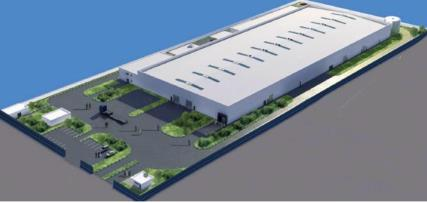
\includegraphics[width=0.68\textwidth]{usine-kenitra.jpg}
  \caption{Vue du site Saint-Gobain Sekurit de Kénitra}
\end{figure}

\begin{table}[H]
\centering
\caption{Fiche synthétique de l'organisme d'accueil}
\begin{tabularx}{0.93\textwidth}{>{\bfseries}p{0.31\textwidth}Y}
\toprule
Élément & Présentation synthétique \\
\midrule
Entreprise & Saint-Gobain Sekurit Maroc \\
Implantation & Atlantic Free Zone, Kénitra \\
Activité & Production de pare-brise automobiles \\
Clients cités & Stellantis, Renault, Volkswagen et Seat \\
Certifications citées & IATF 16949, ISO 9001, ISO 14001 et ISO 45001 \\
Produits présentés & Pare-brise feuilleté, PVB chauffant et PVB antenne \\
\bottomrule
\end{tabularx}
\end{table}

\section{Le pare-brise feuilleté}

Un pare-brise feuilleté associe deux feuilles de verre et un film intermédiaire
en PVB. Ce film maintient les fragments en cas de choc et peut recevoir des
fonctions supplémentaires, comme le chauffage ou une antenne. La fabrication
ne consiste donc pas seulement à découper une forme. Elle enchaîne des
opérations de préparation, d'impression, de bombage, d'assemblage et de
contrôle~\cite{sekuritprocess}.

\begin{figure}[H]
  \centering
  \begin{subfigure}[b]{0.44\textwidth}
    \centering
    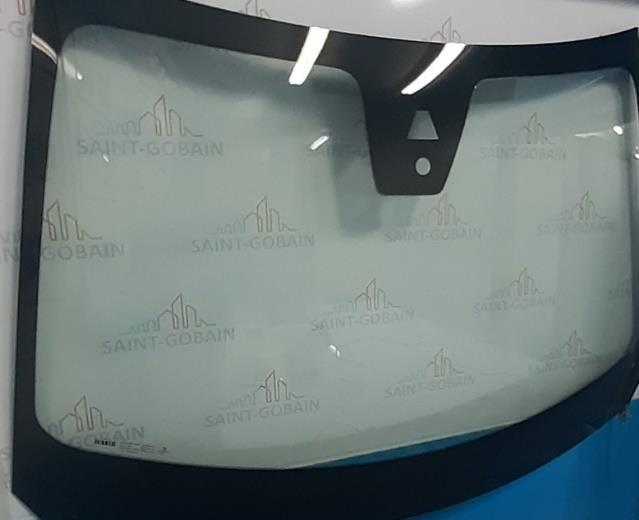
\includegraphics[width=\linewidth,height=5.2cm,keepaspectratio]{pare-brise-feuillete.jpg}
    \caption{Pare-brise feuilleté}
  \end{subfigure}
  \hfill
  \begin{subfigure}[b]{0.50\textwidth}
    \centering
    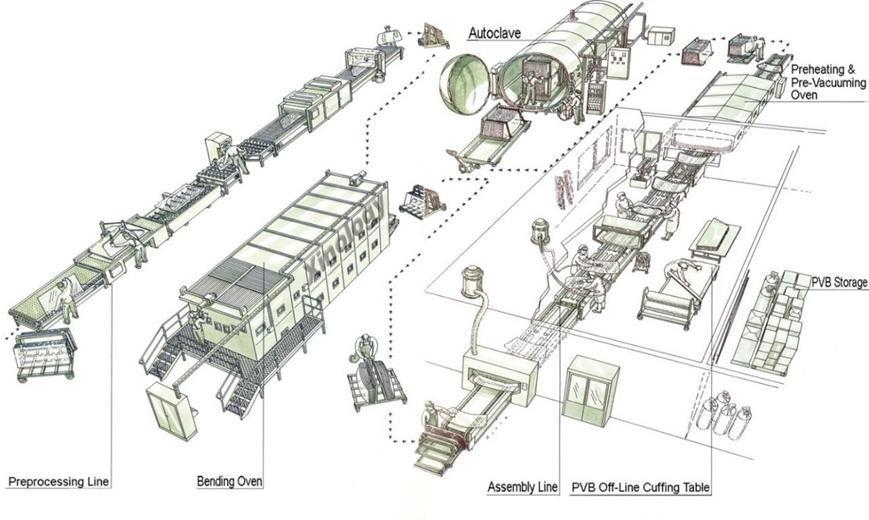
\includegraphics[width=\linewidth,height=5.2cm,keepaspectratio]{procede-verre-feuillete.jpg}
    \caption{Vue d'ensemble du procédé}
  \end{subfigure}
  \caption{Produit et chaîne de fabrication du vitrage automobile}
\end{figure}

\section{Place de l'impression et du contrôle}

Dans la partie pré-processing, le verre est chargé, découpé, façonné, lavé et
imprimé. La sérigraphie du logo et de la bande noire est suivie d'un contrôle
visuel et d'un contrôle automatique. Le projet GlassInk Monitor concerne un
autre équipement d'impression, une
imprimante CIJ dédiée au marquage DMC, mais les enjeux restent proches :
position correcte, contraste suffisant, lisibilité et traçabilité.

\begin{figure}[H]
  \centering
  \begin{subfigure}[b]{0.48\textwidth}
    \centering
    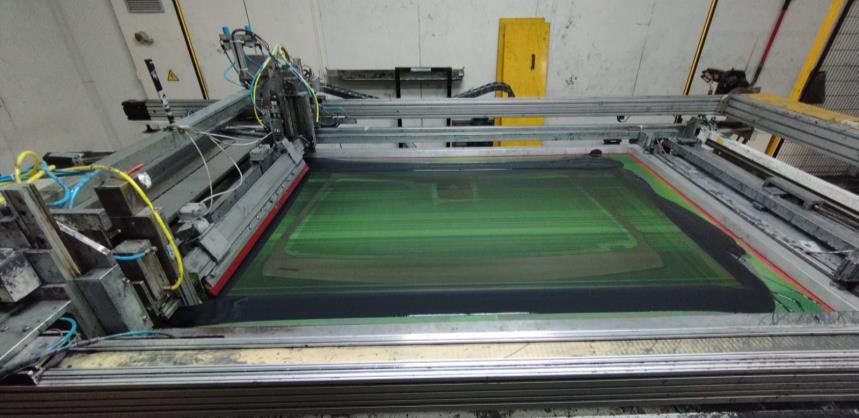
\includegraphics[width=\textwidth]{serigraphie.jpg}
    \caption{Table d'impression sur verre}
  \end{subfigure}
  \hfill
  \begin{subfigure}[b]{0.48\textwidth}
    \centering
    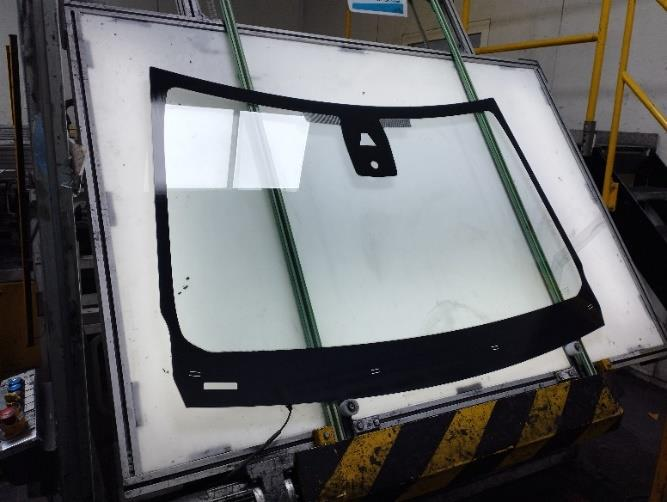
\includegraphics[width=\textwidth]{pare-brise-controle.jpg}
    \caption{Pare-brise au poste de contrôle}
  \end{subfigure}
  \caption{Exemples d'impression et de contrôle dans la ligne}
\end{figure}

Un défaut de marquage peut avoir plusieurs origines. La donnée imprimée peut
être fausse, la machine peut manquer de fluide, la viscosité peut dériver ou la
buse peut être partiellement obstruée. Une supervision utile doit donc réunir
les informations du procédé, de l'imprimante et des consommables.

\section{Systèmes industriels présents}

Les PLC coordonnent les équipements de la ligne et échangent leurs données sur
PROFINET. Litmus Edge récupère les tags industriels, les normalise et peut les
publier vers des systèmes informatiques. Il ne remplace pas les automates :
les automatismes restent responsables du contrôle de la production.

Ce découpage fixe la frontière du projet. GlassInk Monitor commence au niveau
de la sortie MQTT de Litmus Edge. La configuration des drivers PLC et la
logique de commande de la ligne ne font pas partie du travail.

\chapter{Recherche bibliographique et état de l'art}

\section{Démarche de recherche}

Cette étude ne prétend pas être une revue systématique de toute la
littérature sur l'IIoT. Elle répond à une question plus concrète : quelles
solutions permettent de construire une supervision industrielle à partir de
données déjà disponibles sur une plateforme edge ? La recherche a donc suivi
six axes : l'interopérabilité OT/IT, la surveillance conditionnelle, le
transport MQTT, l'ingestion des messages, le stockage temporel et la
visualisation.

Les sources ont été choisies dans un ordre simple. Les normes et
spécifications officielles ont servi pour les protocoles. Les documentations
des éditeurs ont permis de vérifier les possibilités des outils. Enfin, des
articles scientifiques ont été consultés pour situer le projet par rapport à
la maintenance conditionnelle et prédictive. Les critères de sélection ont
été la compatibilité avec Litmus Edge, la possibilité d'un déploiement local,
la lisibilité pour une équipe industrielle et un coût raisonnable pour une
seule ligne.

\section{De la maintenance corrective à la surveillance conditionnelle}

La maintenance corrective intervient après la panne. La maintenance
préventive remplace ou contrôle un équipement selon un calendrier, même si son
état réel ne l'exige pas encore. La maintenance conditionnelle s'appuie au
contraire sur des mesures : température, pression, vibration, niveau,
viscosité ou compteur d'heures. Elle cherche une dérive avant que le défaut ne
bloque la production.

La maintenance prédictive va plus loin. Elle utilise un historique suffisant
pour estimer une probabilité de panne ou une durée de vie restante. La revue
de Krupitzer et al. montre que cette démarche repose sur la collecte, la
préparation et l'interprétation de données industrielles, souvent avec des
méthodes d'apprentissage automatique~\cite{krupitzer2020survey}. Li, Fei et
Zhang décrivent une architecture edge-to-cloud appliquée à la surveillance
d'équipements de fabrication. Le traitement à la périphérie réduit le volume
échangé et rapproche l'analyse de la machine~\cite{li2022condition}.

GlassInk Monitor se place volontairement au niveau de la \textbf{surveillance
conditionnelle}. Le système détecte des seuils, suit des tendances et
extrapole le temps avant épuisement d'un fluide. Il ne prédit pas encore une
panne par apprentissage automatique. Il manque pour cela des mois de données
réelles, des défauts correctement étiquetés et un retour de la maintenance.
Employer dès maintenant le terme de maintenance prédictive donnerait une
image plus ambitieuse, mais techniquement inexacte.

\section{Données disponibles sur la Markem-Imaje 9450c}

La ligne étudiée utilise une imprimante Markem-Imaje 9450c à jet d'encre
continu, adaptée aux cadences industrielles et équipée d'une connectivité
Ethernet~\cite{markem9450}. Elle est raccordée à un automate Siemens
S7-1515-2~PN. La communication s'appuie sur TCP/IP et sur des trames contenant
un identifiant, une longueur, des données utiles et une somme de contrôle.

\begin{figure}[H]
  \centering
  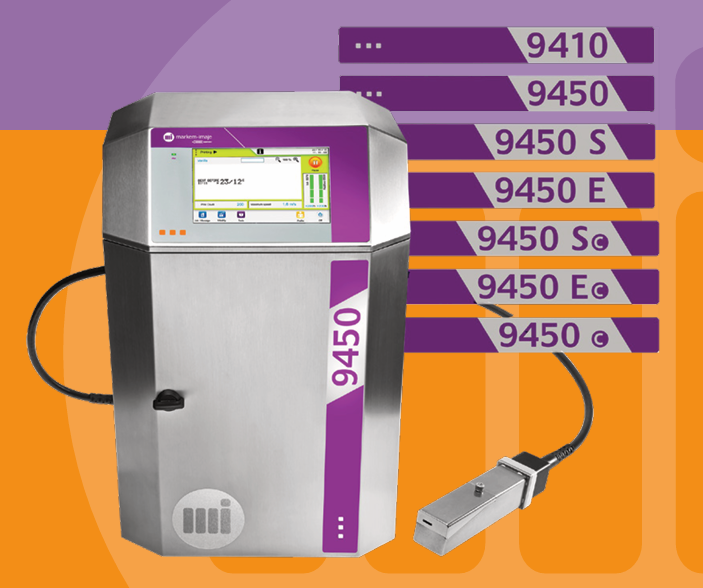
\includegraphics[width=0.66\textwidth]{imprimante-markem-imaje-9450.png}
  \caption{Imprimante CIJ Markem-Imaje 9450 et tête de marquage}
  \label{fig:imprimante-9450}
\end{figure}

Le périmètre de supervision retient huit familles d'informations : alertes,
état général, état de l'impression, état du jet, informations des deux
cartouches, paramètres de fonctionnement et tâche d'impression active.

La réponse des paramètres de fonctionnement contient 84 octets et plus de
quarante valeurs. Parmi elles figurent la vitesse moteur, la pression, la
viscosité, le niveau d'encre, la quantité d'additif injectée, les températures
électronique, encre et tête, les états des électrovannes, le niveau du tube,
l'autonomie d'encre et la consommation moyenne. Les cartouches externes
d'encre et d'additif ont une capacité de 800~mL ; les réservoirs internes ont
une capacité annoncée de 1,075~L et maintiennent une réserve de fonctionnement
d'environ 24~heures. La capacité des cartouches externes et les fonctions de
suivi de l'autonomie sont également indiquées dans la documentation technique
du constructeur~\cite{markem9450}.

Dans l'architecture existante, la 9450c est reliée à Logoface4, puis au système
Gosun. Les données rejoignent ensuite Litmus Edge et l'IoT Backbone. Cette
organisation confirme que la plateforme de
supervision n'a pas à interroger directement l'imprimante : les données déjà
centralisées sur Litmus Edge constituent son point d'entrée. Elle fournit aussi
une base concrète au simulateur, qui reproduit les codes d'état du jet, l'état
d'impression et les paramètres utiles à la maintenance.

\section{Acquisition et interopérabilité à la frontière OT/IT}

Dans une architecture industrielle classique, OPC UA offre un modèle
d'information commun, des services client--serveur et un mode
publication--abonnement. La spécification prévoit aussi l'authentification,
le chiffrement et le contrôle d'intégrité~\cite{opcua}. Une application
pourrait donc lire directement les variables d'un automate ou d'un serveur
OPC UA.

Ce choix n'est pas retenu ici. Les automates, l'imprimante et les équipements
de la ligne sont déjà raccordés à Litmus Edge. La plateforme communique avec
les équipements, conserve des données localement et peut les publier vers
MQTT ou REST~\cite{litmusedge}. Ajouter un second client direct vers les PLC
dupliquerait la collecte et agrandirait inutilement le périmètre de sécurité.
Le point d'entrée de GlassInk Monitor est donc la sortie nord de Litmus Edge.
L'application reste en lecture seule et ne commande aucun équipement.

\section{Transport des données}

MQTT découple la source et les consommateurs. Litmus Edge publie sans connaître
Node-RED, et Node-RED peut redémarrer sans modifier la configuration des
automates. Le QoS~1 retenu garantit une livraison au moins une fois, ce qui
signifie qu'un message peut être reçu deux fois~\cite{mqtt5}. Cette propriété
explique la protection contre les doublons mise en place dans la base.

MQTT ne définit cependant ni le nom des topics industriels ni la structure du
contenu. Sparkplug complète MQTT avec un espace de noms, un format de charge
utile et une gestion de l'état de session adaptée aux usages
IIoT~\cite{sparkplug}. Son format binaire Protobuf demande néanmoins un
décodage supplémentaire.

Pour le prototype, des topics explicites et un contenu JSON ont été choisis.
Ils sont faciles à lire, à simuler et à contrôler pendant une démonstration.
Lors du raccordement, deux cas restent possibles : Litmus Edge publie ce JSON,
ou il publie en Sparkplug B et un décodeur est ajouté à l'entrée du flux.
Cette adaptation ne change ni le modèle des mesures ni les tableaux de bord.

\section{Solutions d'ingestion comparées}

L'ingestion ne consiste pas seulement à copier un message. Elle vérifie le
schéma, sépare télémétrie et événements, rejette les données invalides et
garantit l'idempotence. Trois approches ont été étudiées.

\begin{table}[H]
\centering
\small
\caption{Comparaison des solutions d'ingestion}
\begin{tabularx}{\textwidth}{>{\raggedright\arraybackslash}p{0.17\textwidth}YYY}
\toprule
Solution & Points forts & Limites dans ce projet & Appréciation \\
\midrule
Telegraf &
Configuration déclarative, nombreux plugins, faible consommation. &
Moins souple pour les événements hétérogènes, les remplissages et les
transactions métier. &
Très adapté à des mesures régulières et déjà normalisées. \\
Node-RED &
Flux visuel, adaptation rapide des messages, bonne lisibilité du chemin de
données. &
L'éditeur doit être protégé et les flux doivent rester versionnés et testés. &
Retenu pour le prototype et le raccordement à Litmus Edge. \\
Service spécifique &
Contrôle complet du décodage et des transactions. &
Davantage de code, de maintenance et une logique moins visible pour l'équipe
industrielle. &
À réserver à un besoin que Node-RED ne peut pas couvrir proprement. \\
\bottomrule
\end{tabularx}
\end{table}

Telegraf reste une bonne solution lorsque les messages sont déjà homogènes et
que le chemin entre la source et la base demande peu d'adaptation~\cite{telegraf}.
Ici, la télémétrie, les événements de maintenance et les résultats de marquage
n'ont pas la même structure. Node-RED a donc été retenu pour valider chaque
famille, ajouter les tags utiles et produire le Line Protocol attendu par
InfluxDB. Le flux reste lisible dans l'éditeur tout en étant conservé dans le
dépôt du projet.

\section{Stockage, visualisation et alertes}

InfluxDB organise une donnée autour d'une mesure, de tags indexés, de champs et
d'un horodatage~\cite{influxdb,influxschema}. Ce modèle correspond directement
aux variables de l'imprimante : l'identité de la machine et la ligne deviennent
des tags, tandis que les niveaux, températures et compteurs restent des champs.
Les défauts et les marquages sont conservés dans des mesures distinctes. Cette
séparation évite de multiplier les colonnes lorsque la liste des tags Litmus
évolue.

Le prototype utilise InfluxDB OSS 2.7 avec une organisation et un bucket dédiés.
La durée de rétention du bucket est illimitée pour la démonstration ; elle devra
être fixée avec les équipes qualité et infrastructure avant le raccordement au
site. Node-RED enrichit chaque point avec la classification de la machine et les
prévisions de consommables. Les requêtes Flux filtrent ensuite les séries,
appliquent les fenêtres temporelles et agrègent les indicateurs affichés dans
Grafana~\cite{flux}.

Grafana dispose d'une source InfluxDB native. Elle interroge le bucket en Flux,
construit les vues opérateur, maintenance et direction, puis évalue les règles
d'alerte~\cite{grafanainflux}. Pour une ligne et moins de 200 pièces par heure,
une instance de chaque service suffit. La haute disponibilité pourra être
étudiée à partir de mesures réelles de charge et des exigences du site.

\section{Synthèse et positionnement du projet}

\begin{table}[H]
\centering
\small
\caption{Positionnement de GlassInk Monitor}
\begin{tabularx}{\textwidth}{
  >{\raggedright\arraybackslash}p{0.16\textwidth}
  >{\raggedright\arraybackslash}p{0.25\textwidth}
  >{\raggedright\arraybackslash}p{0.20\textwidth}
  Y}
\toprule
Brique & Options étudiées & Choix & Motif principal \\
\midrule
Point d'intégration &
PLC/OPC UA direct, Litmus Edge &
Litmus Edge &
La collecte industrielle existe déjà. \\
Transport &
MQTT JSON, Sparkplug B &
MQTT JSON au prototype &
Lecture et simulation simples ; décodage Sparkplug ajoutable. \\
Ingestion &
Telegraf, Node-RED, service spécifique &
Node-RED &
Transformation visuelle des mesures et événements. \\
Stockage &
InfluxDB, base relationnelle, stockage par fichiers &
InfluxDB 2.7 &
Modèle temporel natif, rétention et intégration directe avec Grafana. \\
Supervision &
Application web, Grafana &
Grafana &
Tableaux de bord, rôles et alertes déjà disponibles. \\
Déploiement &
Services natifs, Docker Compose, Kubernetes &
Docker Compose &
Reproductible et proportionné à une seule ligne. \\
Niveau d'analyse &
Seuils, surveillance conditionnelle, modèle prédictif &
Surveillance conditionnelle &
Pas encore d'historique réel étiqueté pour entraîner un modèle. \\
\bottomrule
\end{tabularx}
\end{table}

L'état de l'art conduit ainsi à une architecture edge-to-dashboard maîtrisée :
Litmus Edge comme frontière industrielle, MQTT pour le découplage, Node-RED
pour l'adaptation, InfluxDB pour l'historisation et Grafana pour l'usage
quotidien. L'apport du projet tient à la manière dont ces briques répondent au
fonctionnement de la ligne : l'activité dépend de la commande, les fluides
peuvent expirer avant d'être vides et le raccordement final doit rester limité
à la configuration de la source Litmus Edge.

\clearpage
\section{Problématique retenue}

À la suite de cette analyse, la problématique du PFA est formulée ainsi :

\begin{projectbox}
\centering
\emph{Comment transformer les données disponibles sur Litmus Edge en une
supervision fiable de l'imprimante CIJ, capable d'anticiper les ruptures et la
péremption des consommables, de distinguer un arrêt réel d'une période sans
commande et de présenter une information adaptée à chaque utilisateur ?}
\end{projectbox}

Cette question générale se décline en trois questions d'ingénierie :

\begin{enumerate}
  \item comment transporter et enregistrer les messages en tenant compte des
        retransmissions possibles avec le QoS~1 ?
  \item comment calculer la disponibilité sans classer une absence de commande
        comme une panne ?
  \item comment réunir dans une seule décision le temps avant épuisement et la
        date effective de péremption d'un fluide ?
\end{enumerate}

Deux contraintes encadrent la réponse. Le projet ne commande ni l'imprimante
ni les automates : le flux reste en lecture seule. Par ailleurs, l'accès au
Litmus Edge réel n'était pas disponible pendant le développement. La solution
devait donc être construite et vérifiée avec un simulateur, puis rester
remplaçable par la source industrielle sans reprendre toute l'application.

\chapter{Analyse du besoin et cahier des charges}

\section{Situation observée}

La ligne peut produire 24 heures sur 24, cinq jours par semaine. Cela ne veut
pas dire que l'imprimante doit fonctionner en continu. Son utilisation dépend
des commandes et de la référence de pare-brise en cours. Pendant une période
sans demande, une imprimante arrêtée n'est pas en panne. À l'inverse, si un
verre arrive au poste et que l'imprimante est indisponible, le temps perdu doit
être enregistré.

Cette différence paraît simple, mais elle change les indicateurs. Une
disponibilité calculée sur le temps calendaire pénaliserait les périodes sans
commande. Elle produirait des alertes inutiles, puis les utilisateurs
finiraient par les ignorer.

\section{Parties prenantes}

\begin{table}[H]
\centering
\caption{Attentes des utilisateurs}
\begin{tabularx}{\textwidth}{p{0.22\textwidth}YY}
\toprule
Utilisateur & Question principale & Information attendue \\
\midrule
Opérateur &
La machine peut-elle imprimer maintenant ? &
État, niveau des fluides, défaut actif et volume récent. \\
Maintenance &
Pourquoi la machine s'arrête-t-elle et quand intervenir ? &
Tendances, heures restantes, historique, Pareto des défauts et service à prévoir. \\
Direction &
Quel est l'effet sur la production ? &
Disponibilité liée à la demande, temps d'arrêt, rendement et volume marqué. \\
\bottomrule
\end{tabularx}
\end{table}

\section{Exigences fonctionnelles}

\begin{longtable}{p{0.11\textwidth}p{0.58\textwidth}p{0.20\textwidth}}
\caption{Exigences fonctionnelles du prototype}\\
\toprule
Réf. & Exigence & Critère d'acceptation \\
\midrule
\endfirsthead
\toprule
Réf. & Exigence & Critère d'acceptation \\
\midrule
\endhead
F01 & Recevoir les mesures et événements par MQTT. &
Les trois familles de topics sont consommées. \\
F02 & Afficher l'état courant de l'imprimante. &
État mis à jour en moins d'une période de publication. \\
F03 & Suivre les niveaux d'encre et de solvant. &
Courbes, valeur courante et seuils visibles. \\
F04 & Estimer le temps avant épuisement. &
Prévision calculée à partir d'une pente récente. \\
F05 & Gérer la péremption d'un consommable. &
Date imprimée et durée après ouverture comparées. \\
F06 & Distinguer un arrêt réel d'une absence de commande. &
Le signal de demande conditionne l'indicateur. \\
F07 & Enregistrer les défauts et leur durée. &
Historique filtrable et Pareto sur 30 jours. \\
F08 & Conserver le marquage DMC et son résultat de contrôle. &
Recherche par DMC et statistiques de qualité possibles. \\
F09 & Déclencher des alertes. &
Sept règles provisionnées et un webhook testé. \\
F10 & Présenter des vues adaptées aux trois publics. &
Trois tableaux de bord distincts. \\
\bottomrule
\end{longtable}

\section{Exigences non fonctionnelles}

\begin{itemize}
  \item \textbf{Lecture seule :} aucun service du projet n'écrit vers le PLC ou
        l'imprimante.
  \item \textbf{Reproductibilité :} l'environnement complet doit démarrer avec
        Docker Compose.
  \item \textbf{Traçabilité :} chaque message possède un identifiant unique.
  \item \textbf{Résistance aux doublons :} une livraison MQTT répétée ne doit
        pas créer deux mesures ou deux événements.
  \item \textbf{Observabilité :} chaque service expose un contrôle de santé ou
        un état visible dans Docker.
  \item \textbf{Confidentialité :} les mots de passe ne figurent ni dans les
        flux Node-RED ni dans le fichier Compose.
  \item \textbf{Évolutivité raisonnable :} l'ajout d'un tag ne doit pas imposer
        une refonte du modèle de stockage.
\end{itemize}

\section{Périmètre et hypothèses}

Le périmètre s'arrête à la supervision. Les commandes de production, l'ERP, le
MES, le réglage de l'imprimante et l'écriture dans les automates sont exclus.
Le prototype utilise les hypothèses suivantes :

\begin{itemize}
  \item une seule ligne, avec moins de 200 pare-brise par heure ;
  \item une imprimante CIJ Markem-Imaje 9450c ;
  \item un signal \texttt{line\_demanding} indiquant qu'une impression est
        attendue ;
  \item une caméra de contrôle fournissant un résultat et un grade ;
  \item une durée d'utilisation de 90 jours après ouverture pour les fluides.
\end{itemize}

\begin{warningbox}
Ces valeurs servent au développement. Le modèle exact de l'imprimante, la
liste des tags et la durée réelle après ouverture devront être confirmés avec
la documentation du site avant la mise en service.
\end{warningbox}

\section{Choix d'un simulateur}

Attendre l'accès au Litmus Edge aurait bloqué toutes les étapes suivantes. Le
simulateur n'est donc pas un simple générateur de nombres aléatoires. Il
reproduit les situations qui peuvent tromper la supervision : démarrage,
préchauffage, production, attente sans commande, jet laissé actif, défaut,
remplissage, dérive de viscosité et perte temporaire de communication.

Il accélère le temps par un facteur configurable. Une minute réelle peut
représenter une heure simulée. Les tendances et les alertes deviennent ainsi
visibles pendant une démonstration, tout en gardant des horodatages réels dans
la base.

\chapter{Conception de la solution}

\section{Architecture générale}

L'architecture sépare la collecte industrielle, le transport, le traitement,
le stockage et la visualisation. Cette séparation facilite les essais et
permet de remplacer le simulateur par Litmus Edge sans réécrire les tableaux
de bord.

\begin{figure}[H]
  \centering
  \includegraphics[width=\textwidth]{architecture-industrielle.pdf}
  \caption{Architecture fonctionnelle de GlassInk Monitor}
  \label{fig:architecture}
\end{figure}

Le PLC et l'imprimante appartiennent à la couche de contrôle existante.
Litmus Edge fournit le point d'intégration. Mosquitto transporte les messages.
Node-RED vérifie leur structure, les convertit en Line Protocol et les écrit
dans InfluxDB. Grafana interroge ensuite le bucket de supervision.

\section{Choix de la pile technique}

\begin{center}
  \stackicon{python.pdf}{Python\\simulateur}
  \hfill
  \stackicon{eclipsemosquitto.pdf}{Mosquitto\\MQTT}
  \hfill
  \stackicon{nodered.pdf}{Node-RED\\ingestion}
  \hfill
  \stackicon{influxdb.pdf}{InfluxDB\\stockage}
  \hfill
  \stackicon{grafana.pdf}{Grafana\\supervision}
  \hfill
  \stackicon{docker.pdf}{Docker\\déploiement}
\end{center}

\subsection{MQTT et Mosquitto}

MQTT suit le modèle publication/abonnement. Le producteur publie sur un topic,
le courtier distribue le message et les consommateurs s'abonnent aux topics
utiles. Mosquitto a été retenu parce que le volume du projet reste faible et
qu'il fournit les fonctions nécessaires : authentification, ACL, TLS,
persistance et outils de test~\cite{mosquitto}.

Le prototype utilise le QoS 1. Ce niveau garantit une livraison ``au moins une
fois''~\cite{mqtt5}. Il améliore la fiabilité, mais autorise un doublon lors
d'une retransmission. L'application doit donc être idempotente.

\subsection{Node-RED}

Node-RED rend le chemin des données visible dans un éditeur. Ce choix est
adapté au passage du simulateur vers Litmus Edge : le mapping peut être
inspecté et modifié sans cacher le traitement dans un service opaque. Les flux
restent versionnés dans \texttt{flows.json}. L'éditeur est authentifié et les
connexions utilisent les variables d'environnement~\cite{nodered}.

\subsection{InfluxDB}

La plateforme produit surtout des données horodatées : mesures continues,
changements d'état, défauts et résultats de marquage. InfluxDB 2.7 les conserve
dans le bucket \texttt{printer\_monitoring}. Trois mesures structurent le
contenu : \texttt{printer\_telemetry}, \texttt{printer\_event} et
\texttt{marking\_event}. Les identifiants utilisés pour filtrer deviennent des
tags ; les valeurs numériques et descriptives restent des champs
~\cite{influxschema}.

\subsection{Grafana}

Grafana interroge nativement InfluxDB. Il affiche les séries temporelles, les
tableaux et les indicateurs calculés avec Flux. Les règles d'alerte réutilisent
les mêmes données~\cite{grafanainflux}. Les tableaux de bord et
la source de données sont provisionnés par fichiers, ce qui évite une
configuration manuelle lors d'une nouvelle installation.

\subsection{Docker Compose}

Chaque composant tourne dans son conteneur. Le fichier Compose décrit les
services, leurs réseaux, leurs volumes, leurs variables et leurs contrôles de
santé. Cette approche reproduit le même environnement sur un poste de
développement et sur une VM de démonstration~\cite{dockercompose}.

\section{Cycle de vie des données}

\begin{figure}[H]
  \centering
  \includegraphics[width=\textwidth]{pipeline-donnees.pdf}
  \caption{Traitement d'une mesure entre la machine et le tableau de bord}
  \label{fig:pipeline}
\end{figure}

Chaque message reçoit un \texttt{message\_id}. Node-RED contrôle les champs
obligatoires, construit un point InfluxDB puis l'envoie à l'API d'écriture v2.
La clé d'un point associe la mesure, son jeu de tags et son horodatage. Une
retransmission strictement identique réécrit donc le même point au lieu d'en
créer un second~\cite{influxduplicate}. Cette propriété couvre les doublons
attendus avec le QoS~1. L'écriture de plusieurs mesures n'est toutefois pas une
transaction globale ; en cas d'échec partiel, Node-RED rejoue les points avec
les mêmes clés.

\section{Topics MQTT}

\begin{table}[H]
\centering
\caption{Arborescence MQTT du prototype}
\begin{tabularx}{\textwidth}{p{0.27\textwidth}Y}
\toprule
Type & Topic \\
\midrule
Télémétrie &
\texttt{sgx/<site>/<ligne>/printer/<id>/telemetry} \\
Événement &
\texttt{sgx/<site>/<ligne>/printer/<id>/event} \\
Marquage &
\texttt{sgx/<site>/<ligne>/printer/<id>/marking} \\
Rejet &
\texttt{sgx/system/dead-letter} \\
État Node-RED &
\texttt{sgx/system/node-red/status} \\
\bottomrule
\end{tabularx}
\end{table}

Lors du raccordement réel, Litmus Edge pourra publier du JSON dans cette
arborescence ou utiliser Sparkplug B. Dans le second cas, un nœud de décodage
protobuf sera ajouté avant la validation ; le stockage et les tableaux de bord
ne changeront pas.

\section{Modèle de données}

\begin{figure}[H]
  \centering
  \includegraphics[width=0.93\textwidth]{modele-donnees.pdf}
  \caption{Organisation des données dans le bucket InfluxDB}
  \label{fig:model}
\end{figure}

La mesure \texttt{printer\_telemetry} regroupe les valeurs continues sous forme
de champs : niveau d'encre, niveau de solvant, viscosité, températures,
pression et compteurs. \texttt{printer\_event} conserve les changements d'état,
les défauts et les remplissages. \texttt{marking\_event} contient le DMC, le
résultat du contrôle et le grade de lecture. Les tags \texttt{printer\_id},
\texttt{line\_id}, \texttt{event\_type} et \texttt{verify\_grade} permettent les
filtres courants sans transformer chaque valeur numérique en série indexée.
Node-RED ajoute aussi le tag \texttt{classification} et les champs dérivés
\texttt{hours\_to\_empty}, \texttt{action\_days} et
\texttt{expiry\_limited} pour chaque fluide.

\section{Disponibilité liée à la demande}

\begin{figure}[H]
  \centering
  \includegraphics[width=0.92\textwidth]{logique-disponibilite.pdf}
  \caption{Distinction entre production, arrêt et attente normale}
  \label{fig:demand}
\end{figure}

La disponibilité est calculée sur les échantillons où la ligne demande une
impression :

\begin{equation}
A = \frac{N_{\text{demande et marche}}}
         {N_{\text{demande}}}\times 100
\end{equation}

Une période sans commande n'entre ni au numérateur ni au dénominateur. Si le
flux réel est publié à intervalle fixe, ce comptage approche correctement le
temps. Si Litmus publie uniquement lors d'un changement, il faudra reconstruire
des intervalles et pondérer par leur durée.

\section{Prévision et péremption}

Node-RED estime la consommation à partir de deux niveaux successifs. Pour
limiter l'effet du bruit, le débit observé est lissé avec le débit précédent :

\begin{equation}
r_k = 0{,}75\,r_{k-1} + 0{,}25\,
      \frac{L_{k-1}-L_k}{t_k-t_{k-1}}
\end{equation}

Pour un débit $r_k$ exprimé en points de pourcentage par heure et un niveau
courant $L_k$, le temps avant épuisement vaut :

\begin{equation}
T_{\text{vide}} = \frac{L_k}{r_k}
\end{equation}

La date d'action n'est pas forcément déterminée par ce calcul. Un fluide ouvert
peut expirer avant d'être vide. La date effective est :

\begin{equation}
D_{\text{effective}} =
\min\left(D_{\text{imprimée}},
D_{\text{ouverture}} + N_{\text{jours après ouverture}}\right)
\end{equation}

Une hausse supérieure à cinq points indique un remplissage et réinitialise
l'estimation. Le tableau de maintenance affiche les deux échéances et retient
celle qui arrive en premier.

\chapter{Réalisation de la plateforme}

\section{Organisation du projet}

Le dépôt est organisé par service. Chaque dossier contient sa configuration,
son code et un fichier README.

\begin{lstlisting}[language=bash,caption={Organisation des principaux composants}]
.
|-- broker/        # Eclipse Mosquitto
|-- dashboards/    # provisioning et tableaux Grafana
|-- simulator/     # modele Python de l'imprimante
|-- ingestion/     # image et flux Node-RED
|-- notifier/      # diffusion des alertes
|-- docker-compose.yml # services, volumes et initialisation InfluxDB
`-- Makefile
\end{lstlisting}

Les services de base démarrent sans profil. Le simulateur, Node-RED et le
notifier utilisent des profils Compose. La commande \texttt{make demo}
construit et lance l'ensemble.

\section{Simulateur de l'imprimante CIJ}

Le simulateur est écrit en Python. Il contient un état interne, deux
consommables et un générateur de commandes. Son cycle de fonctionnement suit
les états \texttt{shutdown}, \texttt{warmup}, \texttt{running},
\texttt{stopped} et \texttt{fault}. Une loi de Poisson simplifiée déclenche des
défauts à une fréquence configurable.

Le modèle reprend les données documentées pour la 9450c : cartouches externes
de 800~mL, réservoirs internes de 1,075~L, état du jet, état d'impression,
vitesse moteur, pression, viscosité, températures, niveaux et autonomie
d'encre. Les codes natifs sont publiés en parallèle de l'état
fonctionnel utilisé par le tableau de bord. Par exemple, le code jet
\texttt{00h} représente l'arrêt, \texttt{01h} le démarrage et \texttt{07h} le
fonctionnement normal ; l'état d'impression distingue pause, impression
opérationnelle et imprimante non prête.

\begin{table}[H]
\centering
\caption{Comportements reproduits par le simulateur}
\begin{tabularx}{\textwidth}{p{0.34\textwidth}Y}
\toprule
Comportement & Utilité pour les essais \\
\midrule
Périodes de commande et périodes vides &
Vérifier la disponibilité liée à la demande. \\
Consommation d'encre en production &
Tester les tendances et la prévision d'épuisement. \\
Évaporation du solvant avec le jet actif &
Éviter une prévision basée uniquement sur le nombre de pièces. \\
Remplissage avec saut de niveau &
Vérifier le changement de pente et la gestion des lots. \\
Dérive de viscosité &
Déclencher une alerte avant une dégradation visible. \\
Paramètres natifs de la 9450c &
Vérifier le mapping futur des trames constructeur vers Litmus Edge. \\
Défauts avec code et durée &
Alimenter l'historique, le temps d'arrêt et le Pareto. \\
Silence temporaire du producteur &
Tester l'alerte d'absence de données. \\
\bottomrule
\end{tabularx}
\end{table}

Chaque message contient un UUID dans \texttt{message\_id}. Le Last Will MQTT
annonce aussi un arrêt si le client disparaît sans fermeture propre.

\section{Ingestion avec Node-RED}

\begin{figure}[H]
  \centering
  \includegraphics[width=\textwidth]{flux-node-red.pdf}
\caption{Chaîne d'ingestion mise en œuvre avec Node-RED}
  \label{fig:nodered}
\end{figure}

Node-RED contient trois flux de données et un flux de supervision :

\begin{enumerate}
  \item \textbf{Télémétrie} reçoit les valeurs continues, contrôle le payload
        et construit un point \texttt{printer\_telemetry}.
  \item \textbf{Événements} traite les changements d'état, défauts,
        remplissages et annonces de démarrage.
  \item \textbf{Marquages} enregistre le DMC et le résultat de contrôle.
  \item \textbf{Supervision} sonde InfluxDB, expose \texttt{/health} et
        centralise les erreurs.
\end{enumerate}

\begin{figure}[H]
  \centering
  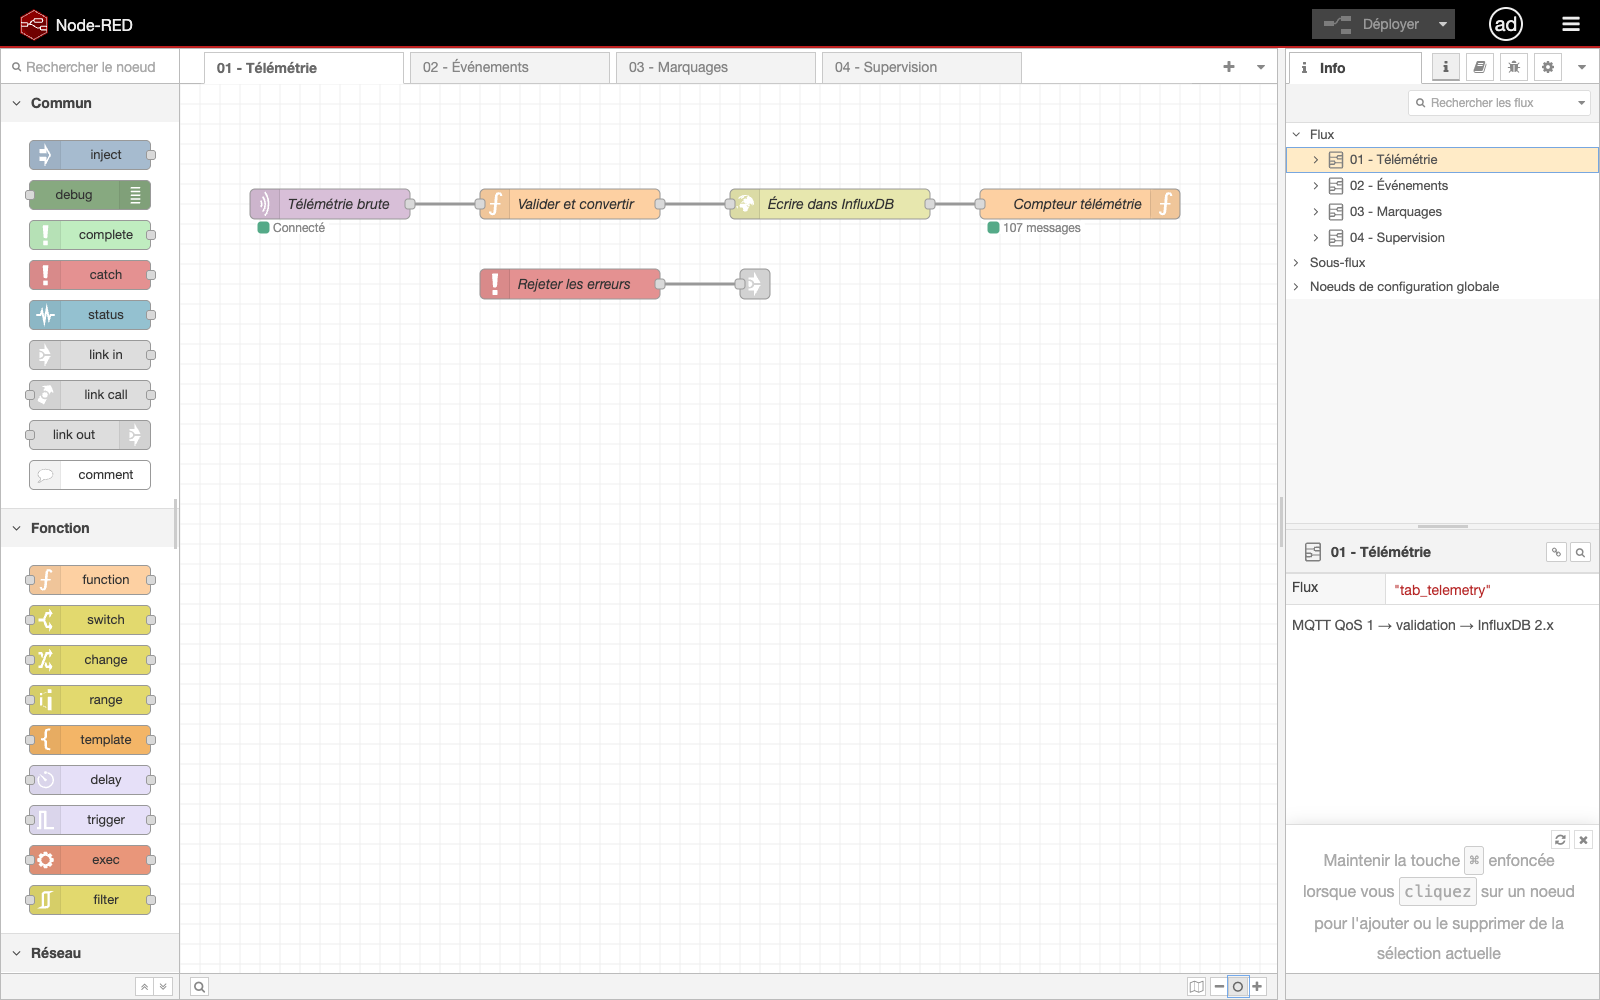
\includegraphics[width=\textwidth]{node-red-telemetrie.png}
  \caption{Flux Node-RED de télémétrie : MQTT, validation et écriture InfluxDB}
  \label{fig:nodered-telemetrie-reel}
\end{figure}

Node-RED utilise un nœud HTTP natif pour appeler directement l'API d'écriture
v2 d'InfluxDB. Aucun module de base de données supplémentaire n'est nécessaire.
Le token, le nom
de l'organisation et le bucket proviennent des variables d'environnement ; ils
ne sont pas inscrits dans \texttt{flows.json}. Le nœud de préparation échappe
les tags et les chaînes avant de produire le Line Protocol :

\begin{lstlisting}[language={},caption={Exemple de Line Protocol produit par Node-RED}]
printer_telemetry,printer_id=CIJ_Printer_L1,line_id=L1 \
ink_level=74.1,solvent_level=57.3,ink_viscosity=4.19 1785445200000
\end{lstlisting}

L'appel HTTP utilise une précision en millisecondes. Il cible l'organisation
\nolinkurl{saint-gobain} et le bucket \nolinkurl{printer_monitoring}. Un message
invalide est publié sur le topic de rejet avec son topic d'origine et un motif
compréhensible par l'exploitant.

\begin{figure}[H]
  \centering
  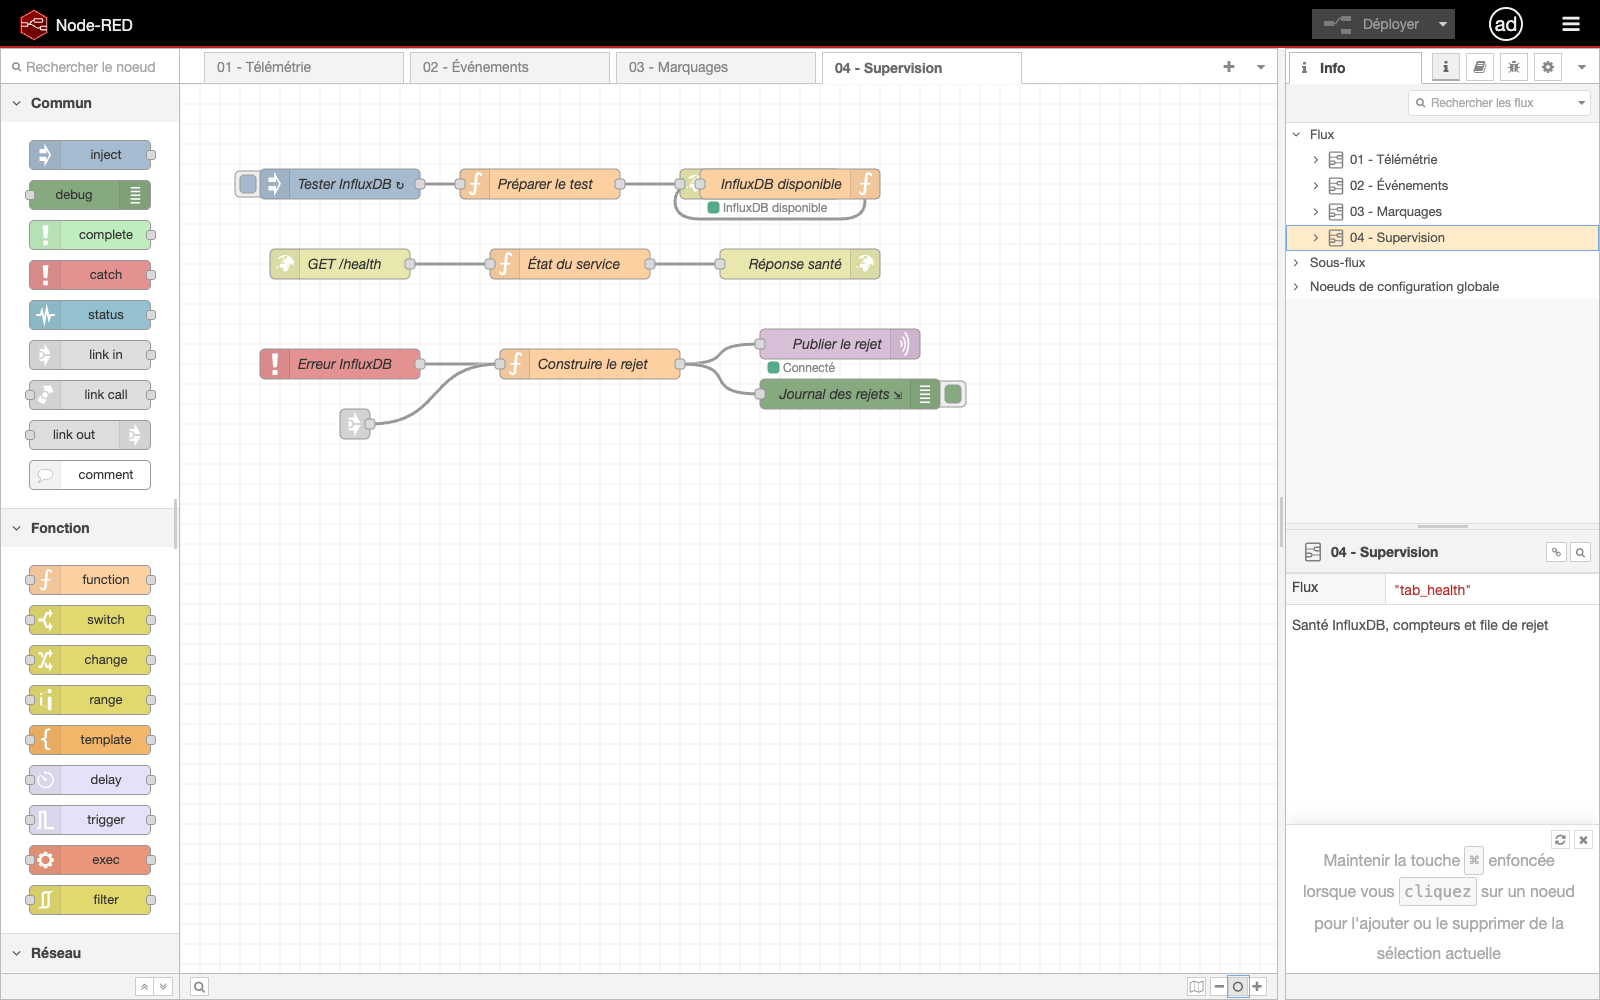
\includegraphics[width=\textwidth]{node-red-supervision.png}
  \caption{Flux Node-RED de supervision et de traitement des rejets}
  \label{fig:nodered-supervision-reel}
\end{figure}

\section{Écriture idempotente et reprise}

InfluxDB identifie un point par sa mesure, ses tags et son horodatage. Le
simulateur conserve l'horodatage d'origine lors d'une retransmission. Node-RED
reconstruit donc la même clé et InfluxDB met à jour le point existant au lieu de
dupliquer l'observation~\cite{influxduplicate}. Le \texttt{message\_id} reste
présent dans les événements pour faciliter le diagnostic, sans être utilisé
comme tag sur la télémétrie afin de limiter la cardinalité.

Une écriture InfluxDB n'offre pas de transaction entre plusieurs mesures. Le
flux traite chaque message de manière indépendante et conserve sa clé lors
d'un nouvel essai. Cette limite est acceptable ici : les messages MQTT sont
autonomes et le rejouage d'un point ne change pas le résultat final.

\section{Requêtes Flux}

Les calculs partagés sont écrits en Flux dans les tableaux de bord et les
règles d'alerte. Ils couvrent notamment :

\begin{itemize}
  \item la dernière valeur de chaque champ de télémétrie ;
  \item la lecture de la classification calculée par Node-RED à partir de la
        demande et de l'état machine ;
  \item la lecture des prévisions d'épuisement et de péremption ajoutées au
        point de télémétrie ;
  \item la disponibilité quotidienne, calculée uniquement pendant la demande ;
  \item le Pareto des défauts et le rendement au premier passage.
\end{itemize}

Les scripts Flux restent dans les fichiers JSON provisionnés de Grafana. Ils
sont contrôlés par la commande \texttt{make verify}, qui exécute les requêtes
contre le bucket de démonstration.

\section{Conteneurisation}

Docker Compose démarre six conteneurs : Mosquitto, InfluxDB, Grafana, le
simulateur, Node-RED et le notifier. Les services attendent la santé de leurs
dépendances. Les données du courtier, d'InfluxDB et de Grafana sont placées
dans des volumes.

Les mots de passe sont générés dans un fichier \texttt{.env} exclu du dépôt.
Le déploiement expose uniquement les interfaces nécessaires aux utilisateurs ;
les services de transport et de stockage restent internes à la plateforme.

\section{Notification des alertes}

Grafana envoie toutes les alertes vers un webhook unique. Le notifier transforme
le payload technique en une phrase courte, puis le transmet aux canaux activés.
Les adaptateurs disponibles sont la console, Telegram, le courrier électronique,
Microsoft Teams et une passerelle WhatsApp de démonstration.

L'adaptateur \texttt{open-wa} n'est pas retenu pour la production. Il pilote
WhatsApp Web, dépend d'une session de téléphone et peut cesser de fonctionner
après une mise à jour. Pour une utilisation industrielle, Teams, l'e-mail ou
l'API WhatsApp Business officielle sont plus faciles à maintenir.

\chapter{Tableaux de bord et alertes}

\section{Principes de présentation}

Un seul tableau de bord pour tous les utilisateurs aurait accumulé les
indicateurs jusqu'à devenir illisible. Trois vues ont donc été créées. Leur
vocabulaire est en français et leurs requêtes renvoient un état explicite
lorsqu'aucune donnée n'est encore disponible.

\section{Vue opérateur}

La vue opérateur doit être comprise rapidement, même à distance. Elle contient
l'état de l'imprimante, le dernier défaut, les niveaux d'encre et de solvant,
le délai avant action et le nombre de pare-brise marqués par période de cinq
minutes.

\begin{table}[H]
\centering
\caption{Correspondance entre état technique et texte affiché}
\begin{tabularx}{0.85\textwidth}{p{0.33\textwidth}Y}
\toprule
Classification & Libellé opérateur \\
\midrule
\texttt{producing} & EN PRODUCTION \\
\texttt{downtime} & À L'ARRÊT \\
\texttt{idle\_jet\_on} & EN ATTENTE \\
\texttt{idle\_no\_order} & SANS COMMANDE \\
absence de mesure & AUCUNE DONNÉE \\
\bottomrule
\end{tabularx}
\end{table}

Le dernier défaut est traduit en français dans la requête. S'il n'existe
aucun défaut, le panneau affiche ``Aucun défaut'' au lieu de ``No data''.

\begin{figure}[H]
  \centering
  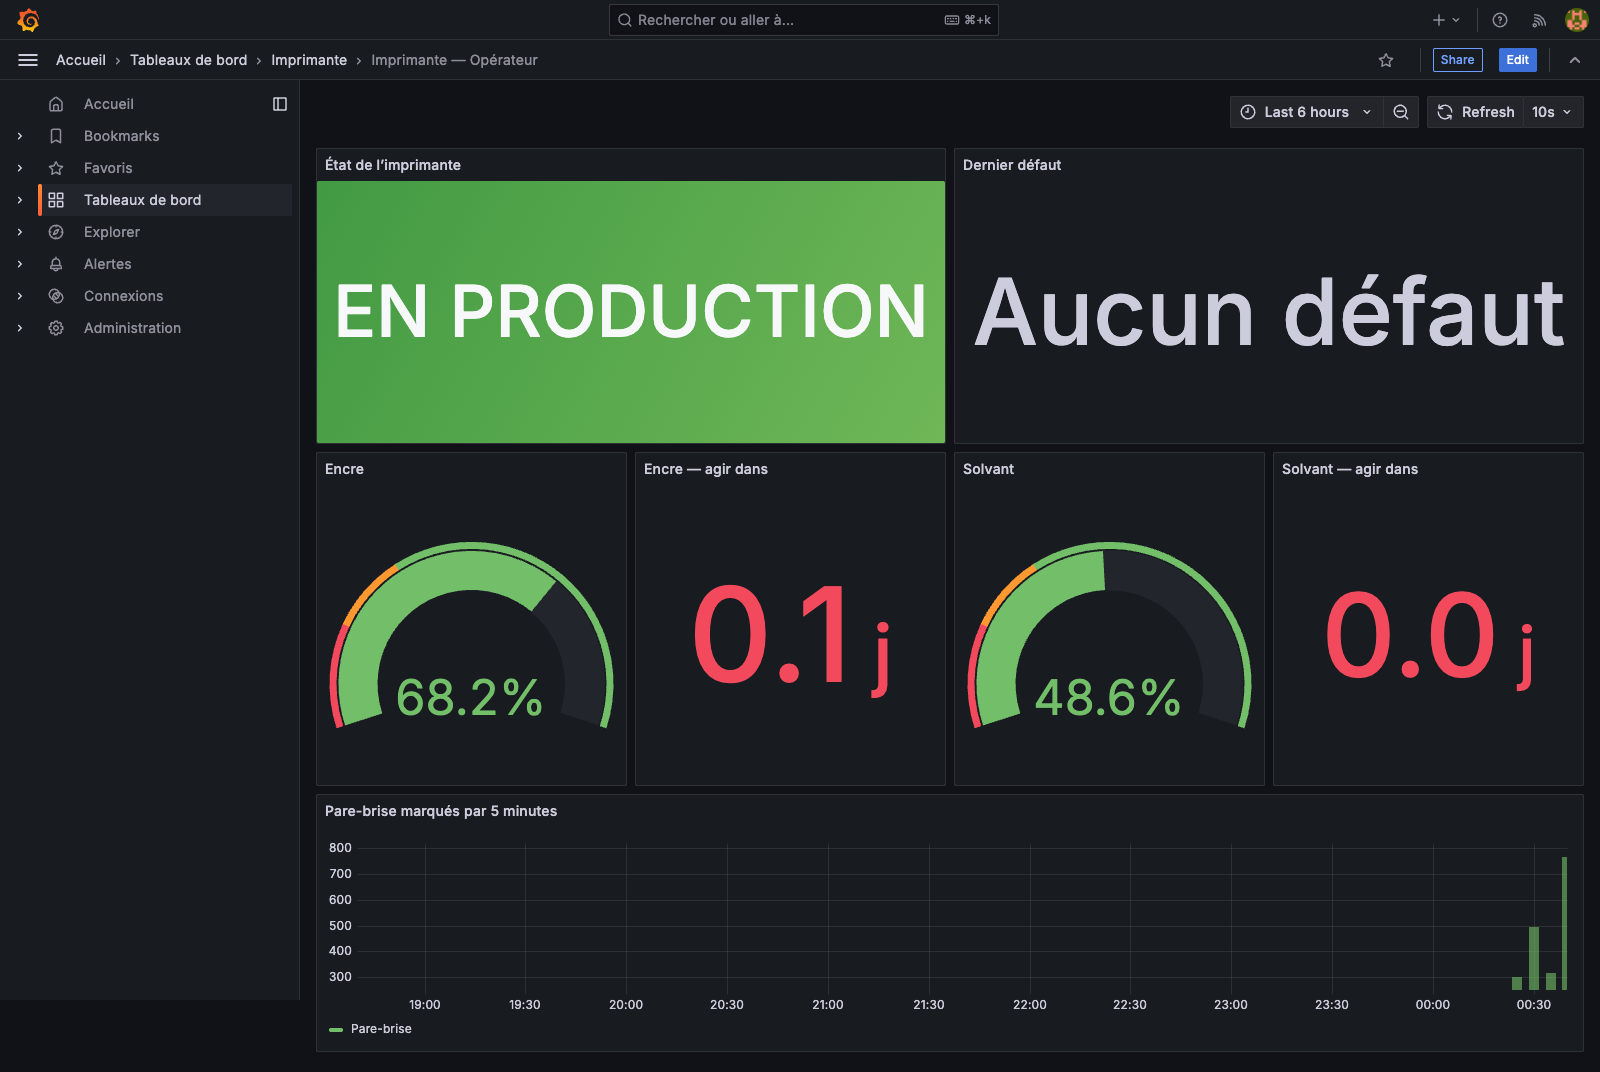
\includegraphics[width=\textwidth]{grafana-operateur.png}
  \caption{Tableau de bord opérateur alimenté par la simulation}
  \label{fig:grafana-operateur}
\end{figure}

\section{Vue maintenance}

La vue maintenance rassemble les informations nécessaires à un diagnostic :

\begin{itemize}
  \item codes natifs du jet et de l'impression, vitesse moteur, pression et
        viscosité générés par le simulateur 9450c ;
  \item capacités de 800~mL et 1,075~L, réserve interne de 24~heures et
        températures électronique, encre et tête ;
  \item tableau des consommables avec lot, niveau, jours avant épuisement,
        date effective de péremption et facteur limitant ;
  \item courbes d'encre et de solvant ;
  \item viscosité comparée à la consigne ;
  \item pression et température de la tête ;
  \item heures restantes avant service ;
  \item liste des défauts récents ;
  \item Pareto du temps perdu par code de défaut ;
  \item historique des lots installés.
\end{itemize}

Le tableau des consommables met côte à côte les deux échéances. Une cartouche
peut être encore remplie à 60~\% et devoir être remplacée cinq jours plus tard
à cause de sa date après ouverture. Afficher uniquement le niveau masquerait ce
cas.

\begin{figure}[H]
  \centering
  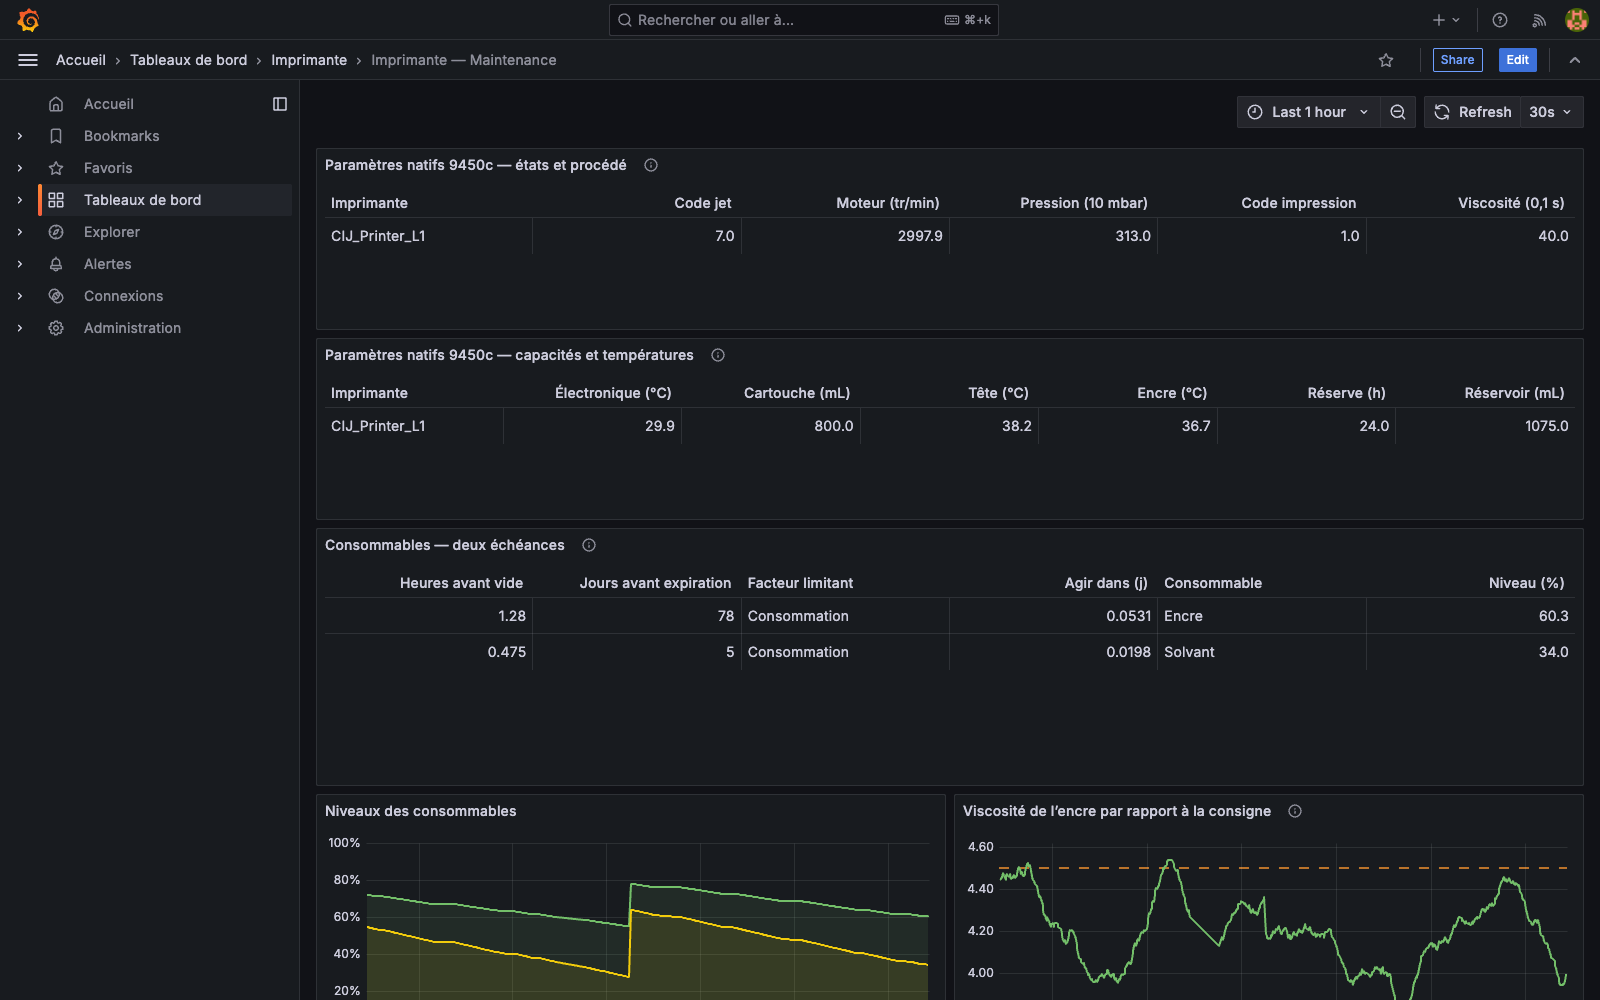
\includegraphics[width=\textwidth]{grafana-simulation-9450c.png}
  \caption{Paramètres natifs produits en direct par la simulation 9450c}
  \label{fig:grafana-simulation-9450c}
\end{figure}

\begin{figure}[p]
  \centering
  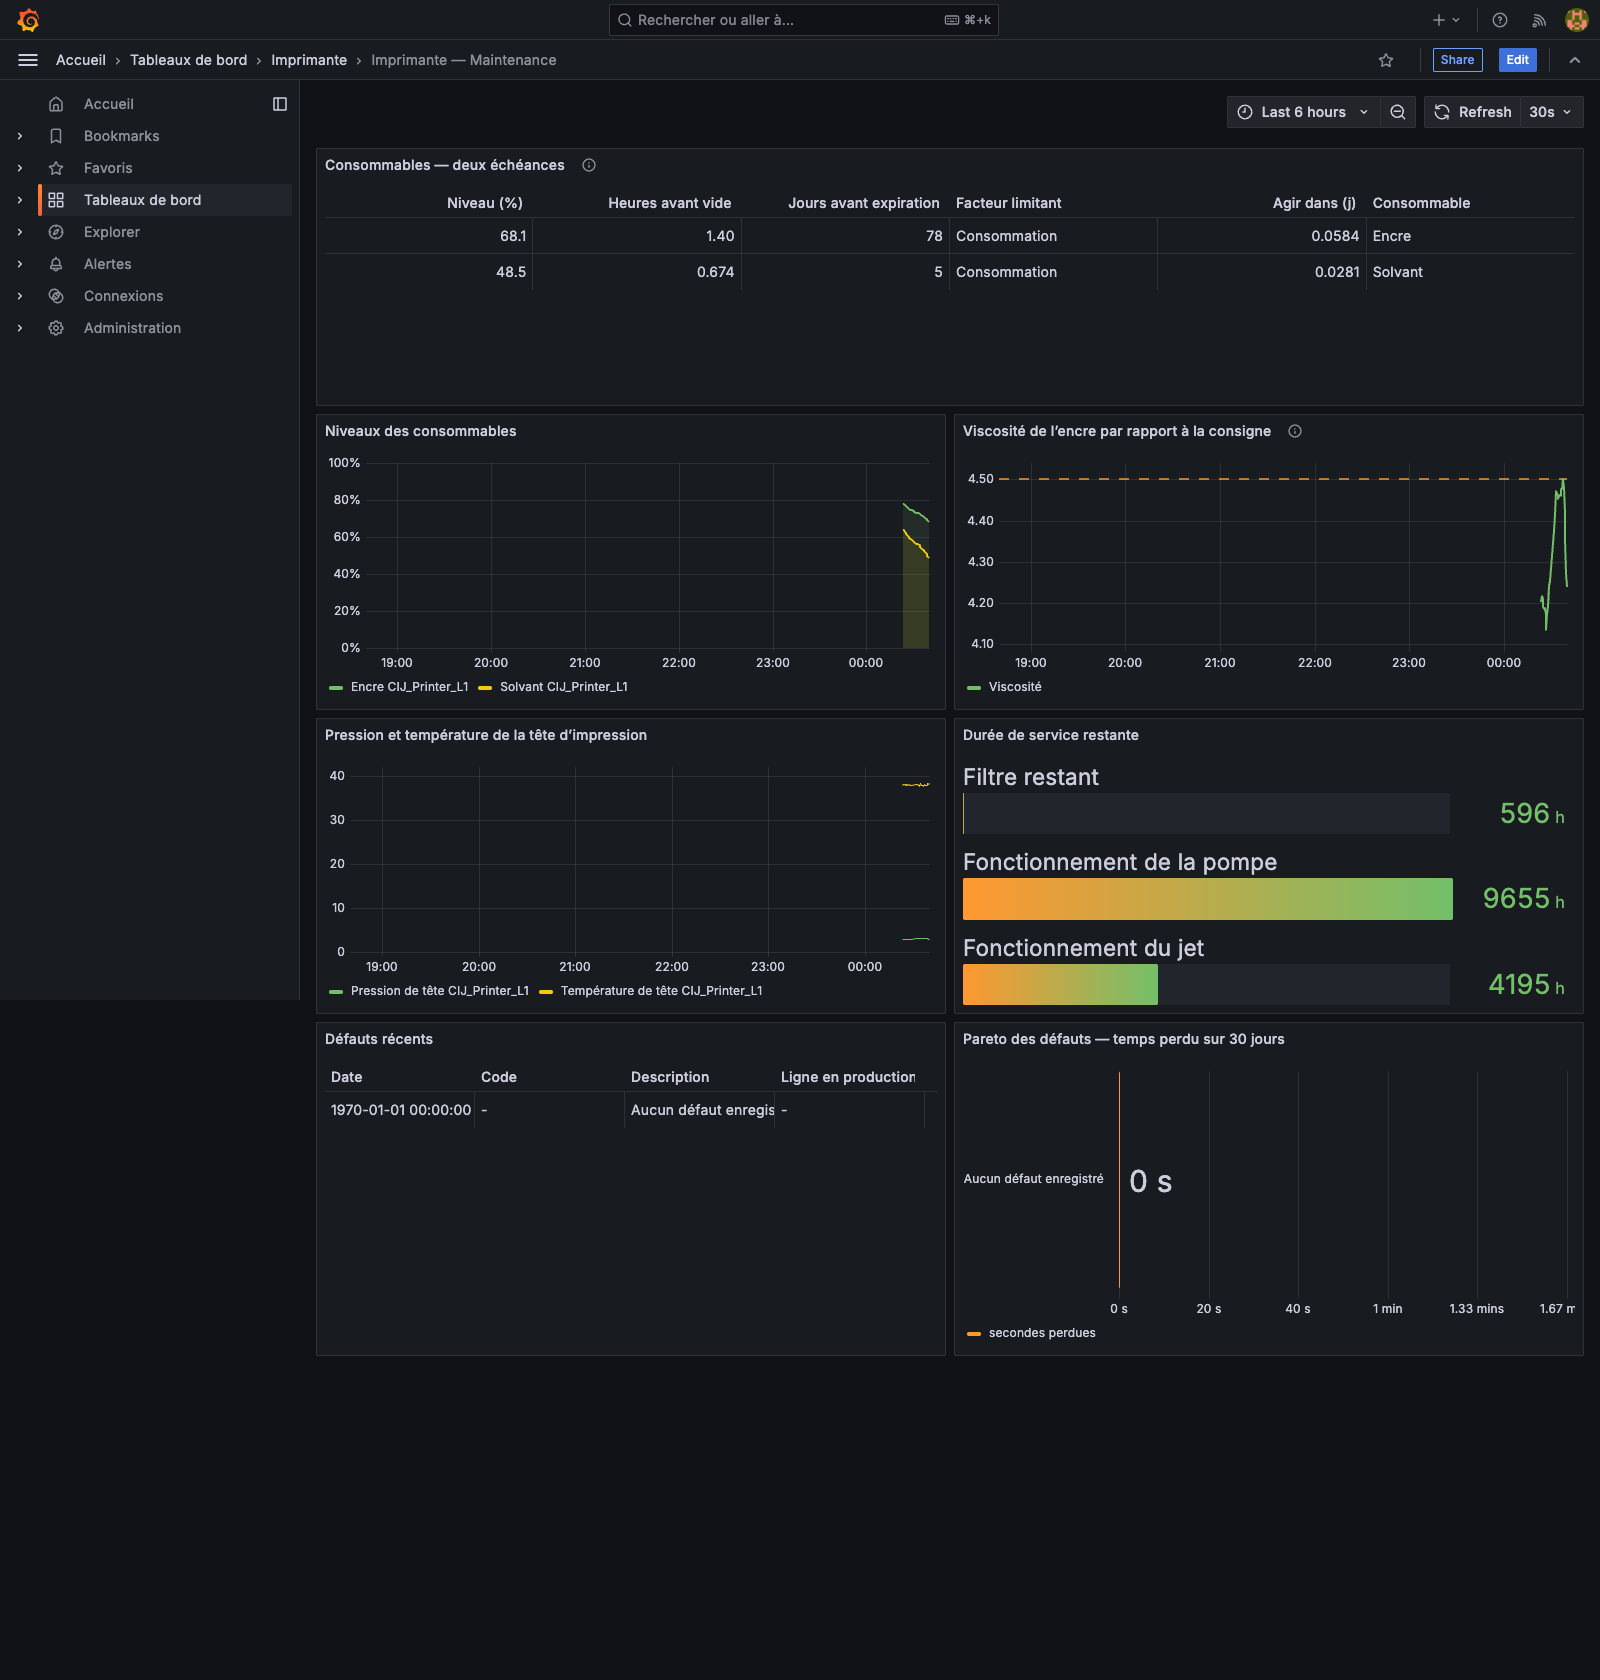
\includegraphics[width=\textwidth,height=0.78\textheight,keepaspectratio]{grafana-maintenance.png}
  \caption{Tableau de bord de maintenance alimenté par la simulation 9450c}
  \label{fig:grafana-maintenance}
\end{figure}

\section{Vue direction}

La vue direction évite les mesures brutes. Elle présente la disponibilité du
jour, le nombre de pare-brise marqués, le rendement au premier passage, le
temps d'arrêt, la répartition du temps et les principales causes d'arrêt. Le
graphique de répartition conserve une catégorie ``sans commande'', car cette
information explique la différence entre temps calendaire et temps demandé.

Si aucune demande n'a encore été observée dans la journée, le panneau de
disponibilité affiche ``NON CALCULÉE''. Une valeur de 0~\% aurait une autre
signification : la ligne aurait demandé des impressions sans aucune
production.

\begin{figure}[H]
  \centering
  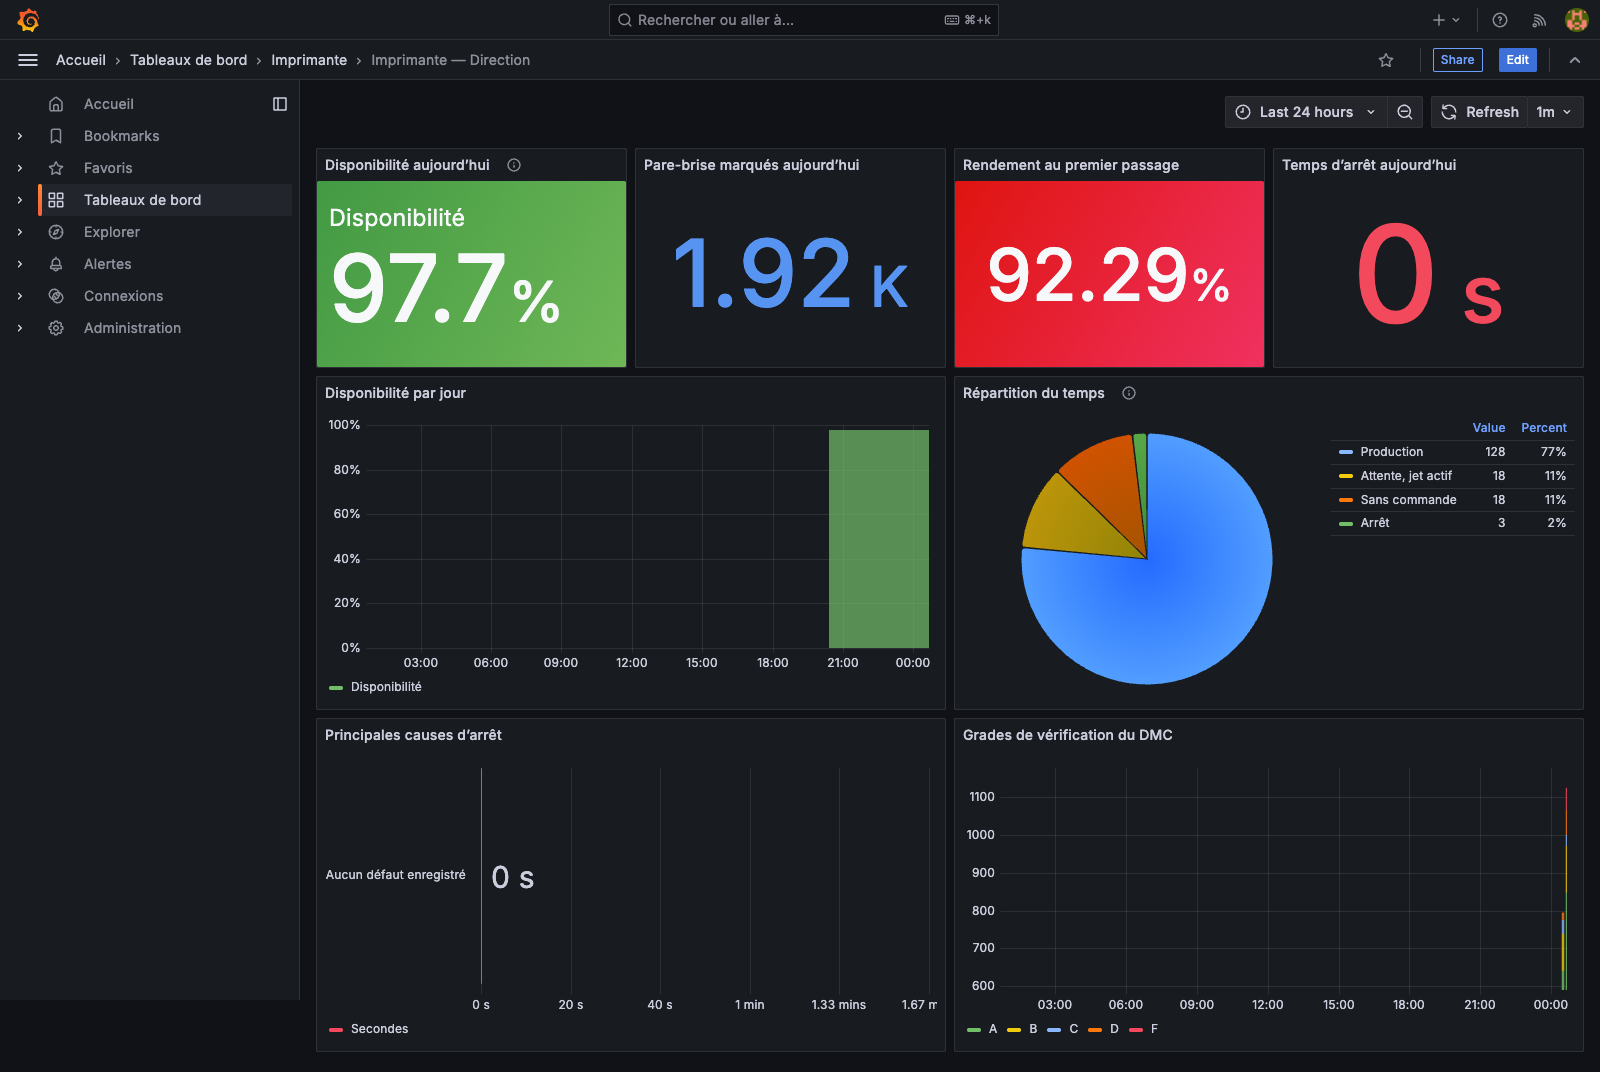
\includegraphics[width=\textwidth]{grafana-direction.png}
  \caption{Tableau de bord de direction alimenté par les données simulées}
  \label{fig:grafana-direction}
\end{figure}

\section{Règles d'alerte}

\begin{longtable}{p{0.29\textwidth}p{0.45\textwidth}p{0.18\textwidth}}
\caption{Règles provisionnées dans Grafana}\\
\toprule
Alerte & Condition & Destinataire \\
\midrule
\endfirsthead
\toprule
Alerte & Condition & Destinataire \\
\midrule
\endhead
Consommable bientôt vide &
Temps estimé inférieur à 8 heures pendant 5 minutes &
Maintenance \\
Niveau bas &
Niveau inférieur à 20~\% pendant 5 minutes &
Maintenance \\
Consommable proche de la péremption &
Moins de 14 jours avant la date effective &
Maintenance \\
Consommable périmé &
Date effective dépassée &
Maintenance et qualité \\
Arrêt avec demande &
Classification \texttt{downtime} pendant 2 minutes &
Opérateur \\
Viscosité hors plage &
Écart supérieur à 0,3 pendant 15 minutes &
Maintenance \\
Absence de données &
Dernière mesure reçue depuis plus de 120 secondes &
Ingénierie \\
\bottomrule
\end{longtable}

Les alertes liées à l'arrêt utilisent le signal de demande. En revanche,
l'absence totale de télémétrie reste un incident, même sans commande : elle
peut indiquer une perte de communication ou un service arrêté.

\section{Lisibilité et langue}

Les titres et les états visibles ont été traduits en français. Les noms de
mesures, champs et codes de défaut restent techniques, car ils servent de
contrat avec l'ingestion. La traduction intervient au niveau de la requête ou
de l'affichage, sans modifier la donnée brute.

Les figures~\ref{fig:grafana-operateur} à~\ref{fig:grafana-direction}
présentent les vues de l'instance Grafana de démonstration alimentée par les
données InfluxDB. Les panneaux disposent d'un état de repli explicite afin de
ne pas confondre une absence de défaut avec une absence de données.

\chapter{Validation du prototype}

\section{Stratégie de test}

La validation combine des tests unitaires et des essais sur la plateforme
complète. Les tests unitaires vérifient les règles du simulateur et le format
des notifications. Les essais d'intégration publient de vrais messages dans
Mosquitto, passent par Node-RED et contrôlent les points écrits dans InfluxDB.
Enfin, les requêtes Flux de chaque panneau sont exécutées par l'API de Grafana.

\section{Tests unitaires}

Douze tests automatisés sont présents :

\begin{itemize}
  \item huit tests du simulateur : identité des messages, date effective de
        péremption, consommation en attente, capacités des fluides, codes et
        paramètres 94xx, débit de marquage et absence de marquage sans demande ;
  \item quatre tests du notifier : format d'une alerte active, regroupement,
        résolution et protection contre un template Grafana non résolu.
\end{itemize}

La commande \texttt{make verify} exécute ces tests, vérifie la syntaxe Compose,
le JSON des flux Node-RED et les fichiers des tableaux de bord.

\section{Essais d'intégration}

\begin{table}[H]
\centering
\caption{Résultats des essais de bout en bout}
\begin{tabularx}{\textwidth}{p{0.31\textwidth}Yp{0.16\textwidth}}
\toprule
Essai & Observation & Résultat \\
\midrule
Publication simulée &
Télémétrie, événements et marquages présents dans le bucket. &
Conforme \\
Message QoS 1 publié deux fois &
Le nombre de points reste inchangé après la retransmission exacte. &
Conforme \\
Payload sans \texttt{message\_id} &
Message reçu sur \texttt{sgx/system/dead-letter} avec le motif. &
Conforme \\
Redémarrage Node-RED &
Reconnexion MQTT puis reprise des écritures. &
Conforme \\
Authentification Node-RED &
\texttt{/flows} renvoie HTTP 401 sans session ; les quatre onglets sont
accessibles après connexion. &
Conforme \\
Source Grafana &
Connexion InfluxDB déclarée saine et bucket accessible. &
Conforme \\
Tableaux de bord &
25 requêtes de panneaux exécutées avec succès. &
Conforme \\
Alertes &
Sept règles chargées depuis les fichiers de provisioning. &
Conforme \\
\bottomrule
\end{tabularx}
\end{table}

\begin{resultbox}
Au terme des essais, les six conteneurs étaient déclarés sains. Les trois
mesures InfluxDB contenaient des points issus du simulateur, et la répétition
d'un message conservait le même résultat. Le prototype valide donc la chaîne
simulateur--MQTT--Node-RED--InfluxDB--Grafana.
\end{resultbox}

\section{Cas de la disponibilité}

Le simulateur alterne les périodes de commande et les périodes vides. Les
échantillons sont classés dans quatre catégories : production, arrêt réel,
attente avec jet actif et absence de commande. Le tableau de bord ne compte
que la deuxième catégorie comme arrêt.

Cet essai a révélé une limite connue. La requête quotidienne compte des
échantillons et suppose une publication périodique. Ce calcul est correct pour
le simulateur. Si Litmus Edge publie seulement lors d'un changement de valeur,
les états longs et courts auraient le même poids. La validation sur site devra
donc vérifier le mode de publication.

\section{Cas des consommables}

Le lot de solvant initial est ouvert depuis 85 jours, avec une durée
configurée de 90 jours après ouverture. Sa date imprimée est plus éloignée,
mais la requête calcule cinq jours restants. Ce scénario vérifie que la plateforme
retient la première échéance.

Les remplissages produisent un saut de niveau. Lorsque la hausse dépasse cinq
points, Node-RED réinitialise le débit estimé. Le délai avant épuisement reste
alors vide jusqu'à la réception d'une nouvelle baisse mesurable, au lieu
d'afficher une prévision négative ou héritée de l'ancienne cartouche.

Les tests de conformité 94xx contrôlent aussi la capacité de 800~mL des
cartouches externes, la capacité de 1,075~L des réservoirs internes et les codes
du jet. Un état \texttt{running} avec demande produit ainsi un code jet 7 et un
état d'impression 1, tandis que la phase de démarrage produit le code jet 1.

\section{Limites de la validation}

Le prototype ne prouve pas encore la compatibilité avec les tags réels de
l'imprimante. Il ne mesure pas non plus la latence du réseau industriel ni la
qualité d'un payload Sparkplug B fourni par le site. Les défauts simulés sont
plausibles, mais leurs codes ne remplacent pas le manuel du modèle installé.

Ces limites ne remettent pas en cause les composants en aval. Elles définissent
le travail de raccordement : capturer un payload réel, établir la table de
mapping, vérifier les unités et rejouer les tests d'acceptation.

\chapter{Sécurité et préparation du déploiement}

\section{Constat réseau}

Les informations disponibles indiquent qu'aucun pare-feu ne sépare actuellement
la plateforme envisagée du réseau des automates. Cette situation augmente le
risque : une erreur de configuration pourrait rendre un service accessible
depuis une zone qui n'en a pas besoin.

\begin{figure}[H]
  \centering
  \includegraphics[width=\textwidth]{deploiement-securite.pdf}
  \caption{Déploiement proposé et mesures à appliquer avant le raccordement}
  \label{fig:security}
\end{figure}

\section{Mesures intégrées au prototype}

\begin{itemize}
  \item les services du projet ne commandent aucun équipement industriel ;
  \item Node-RED, InfluxDB, Mosquitto et le notifier sont liés à l'interface
        locale dans l'environnement de développement ;
  \item l'éditeur Node-RED demande un identifiant et un mot de passe ;
  \item les secrets restent dans \texttt{.env}, avec des permissions de fichier
        limitées ;
  \item Mosquitto possède un exemple de configuration TLS avec comptes séparés
        et ACL ;
  \item le flux Node-RED ne contient pas le token InfluxDB ;
  \item les messages invalides sont isolés dans un journal de rejet.
\end{itemize}

\section{Mesures requises sur site}

Avant toute connexion à Litmus Edge, plusieurs actions sont nécessaires :

\begin{enumerate}
  \item placer la VM de supervision dans un VLAN défini avec le responsable du
        réseau industriel ;
  \item appliquer un pare-feu hôte avec une politique de refus par défaut ;
  \item autoriser uniquement les connexions nécessaires entre Litmus Edge, le
        courtier et les interfaces utilisateur ;
  \item activer TLS pour MQTT et utiliser un certificat délivré ou approuvé par
        l'entreprise ;
  \item créer un compte MQTT par client et limiter ses topics ;
  \item créer un token InfluxDB en lecture seule pour Grafana et un token
        d'écriture distinct pour Node-RED ;
  \item intégrer Grafana à l'identité d'entreprise si elle est disponible ;
  \item sauvegarder le volume InfluxDB et tester une restauration sur une machine
        distincte.
\end{enumerate}

\section{Politique MQTT}

Litmus Edge doit pouvoir publier dans son espace de topics. Node-RED doit lire
ces topics et publier uniquement les rejets et son état. Grafana n'a pas besoin
d'accéder au courtier. Cette séparation réduit les droits de chaque service.

\begin{lstlisting}[caption={Extrait d'ACL MQTT de production}]
user litmus_edge
topic write sgx/<site>/#

user node_red
topic read sgx/<site>/#
topic write sgx/system/dead-letter
topic write sgx/system/node-red/status
\end{lstlisting}

\section{Données et conservation}

Le volume annoncé, inférieur à 200 pièces par heure sur une ligne, reste
modeste. Le prototype conserve tous les événements et compresse les mesures
anciennes. L'entreprise n'a pas encore fourni de durée officielle de
conservation. Cette durée devra être définie avec la qualité et la sécurité des
systèmes d'information avant la production.

Les sauvegardes doivent couvrir le volume InfluxDB, les volumes Grafana utiles
et les fichiers de configuration versionnés. Une sauvegarde qui n'a jamais été
restaurée ne constitue pas une preuve de reprise.

\chapter{Conclusion générale}

GlassInk Monitor transforme des données industrielles dispersées en une chaîne
de supervision cohérente. Le prototype reçoit les messages MQTT, les valide
dans Node-RED, les convertit en Line Protocol, les historise dans InfluxDB et
les présente dans trois tableaux de bord Grafana. Il suit l'état de l'imprimante,
les consommables, les défauts et le résultat des marquages.

Le point le plus délicat n'a pas été l'affichage d'une jauge. Il a été de
définir ce qu'est réellement un arrêt. Sur une ligne qui fonctionne selon les
commandes, une machine immobile n'est pas forcément indisponible. L'ajout d'un
signal de demande rend les indicateurs et les alertes crédibles. La comparaison
entre épuisement et péremption répond au même principe : un pourcentage seul ne
suffit pas pour décider quand intervenir.

Le recours au simulateur a permis d'avancer sans accès au Litmus Edge. Il a
fourni des périodes sans commande, des défauts, des remplissages et des pertes
de communication. Les essais ont validé les doublons MQTT, le journal de rejet,
la reprise après redémarrage, les 23 requêtes de tableaux de bord et les sept
règles d'alerte.

Le projet n'est pas encore raccordé à la production. La prochaine étape est
précise : obtenir un payload Litmus et la liste des tags, confirmer le modèle
de l'imprimante et les unités, puis remplacer le mapping du simulateur. Cette
phase devra aussi valider la sécurité du réseau, le TLS, les ACL, les comptes
Grafana et la sauvegarde.

Ce PFA m'a permis de relier plusieurs domaines de ma formation : réseaux
industriels, messagerie IoT, bases de données temporelles, conteneurisation et
supervision. Il m'a surtout appris qu'un indicateur industriel n'est utile que
si sa définition correspond au fonctionnement réel de la ligne.

\appendix
\chapter{Contrats de messages}

\section{Exemple de télémétrie}

\begin{lstlisting}[language={},caption={Payload de télémétrie publié par le simulateur}]
{
  "message_id": "4efc62a318f84e36bb78cc1341a88b3d",
  "ts": 1785445200000,
  "printer_id": "CIJ_Printer_L1",
  "line_id": "L1",
  "metrics": {
    "printer_state_code": 2,
    "jet_status_code": 7,
    "printing_status_code": 1,
    "jet_running": 1,
    "line_demanding": 1,
    "ink_level": 74.1,
    "solvent_level": 57.3,
    "ink_viscosity": 4.19,
    "head_pressure": 3.02,
    "head_temperature": 38.4,
    "motor_speed_rpm": 2998.0,
    "pressure_10mbar": 302,
    "viscosity_tenth_second": 42,
    "print_count": 184215
  }
}
\end{lstlisting}

\section{Exemple d'événement de remplissage}

\begin{lstlisting}[language={},caption={Payload créant un nouveau lot de solvant}]
{
  "message_id": "a72ba6534dc84b1a95ff5d182d653458",
  "ts": 1785445200000,
  "printer_id": "CIJ_Printer_L1",
  "event_type": "refill",
  "consumable_type": "solvent",
  "part_number": "MI-9876-S",
  "batch_code": "LOT-B12",
  "manufactured_on": "2026-01-15",
  "expires_on": "2027-01-15",
  "opened_on": "2026-07-30",
  "shelf_life_after_open_days": 90,
  "volume_ml": 800
}
\end{lstlisting}

\section{Dictionnaire de la télémétrie}

Le tableau suivant constitue le contrat interne utilisé par les flux et les
tableaux de bord. Les valeurs réelles devront être reliées à ce contrat au
niveau du mapping Litmus Edge--Node-RED.

{\small
\renewcommand{\arraystretch}{1.35}
\begin{longtable}{p{0.34\textwidth}p{0.11\textwidth}p{0.10\textwidth}p{0.30\textwidth}}
\caption{Principaux champs de \texttt{printer\_telemetry}}\\
\toprule
Champ & Type & Unité & Signification \\
\midrule
\endfirsthead
\toprule
Champ & Type & Unité & Signification \\
\midrule
\endhead
\nolinkurl{printer_state_code} & entier & -- & État fonctionnel interne \\
\nolinkurl{jet_status_code} & entier & code & État natif du jet \\
\nolinkurl{printing_status_code} & entier & code & Pause, impression ou non-prêt \\
\nolinkurl{jet_running} & booléen & -- & Jet d'encre actif \\
\nolinkurl{line_demanding} & booléen & -- & Impression attendue par la ligne \\
\texttt{ink\_level} & réel & \% & Niveau d'encre disponible \\
\texttt{solvent\_level} & réel & \% & Niveau de solvant disponible \\
\texttt{ink\_viscosity} & réel & unité machine & Mesure de viscosité utilisée par l'alerte \\
\texttt{head\_pressure} & réel & bar & Pression au niveau du circuit d'encre \\
\texttt{pressure\_10mbar} & entier & 10 mbar & Représentation native de la pression \\
\texttt{head\_temperature} & réel & $^{\circ}$C & Température de la tête \\
\texttt{ink\_temperature} & réel & $^{\circ}$C & Température de l'encre \\
\texttt{electronic\_temperature} & réel & $^{\circ}$C & Température de l'électronique \\
\texttt{motor\_speed\_rpm} & réel & tr/min & Vitesse instantanée du moteur \\
\nolinkurl{motor_speed_target_rpm} & réel & tr/min & Consigne de vitesse du moteur \\
\texttt{print\_count} & entier & pièces & Compteur cumulé d'impressions \\
\texttt{jet\_run\_hours} & réel & h & Durée cumulée de fonctionnement du jet \\
\texttt{pump\_run\_hours} & réel & h & Durée cumulée de fonctionnement de la pompe \\
\nolinkurl{filter_hours_remaining} & réel & h & Durée avant service du filtre \\
\texttt{ink\_tank\_level\_mm} & réel & mm & Hauteur simulée du réservoir interne \\
\texttt{additive\_tank\_level\_mm} & réel & mm & Hauteur simulée du réservoir d'additif \\
\texttt{ink\_internal\_tank\_ml} & réel & mL & Volume interne d'encre estimé \\
\addlinespace[4pt]
\nolinkurl{additive_internal_tank_ml} & réel & mL & Volume interne d'additif estimé \\
\addlinespace[4pt]
\nolinkurl{external_cartridge_capacity_ml} & réel & mL & Capacité nominale de la cartouche \\
\nolinkurl{internal_tank_capacity_ml} & réel & mL & Capacité nominale du réservoir interne \\
\texttt{internal\_reserve\_hours} & réel & h & Réserve interne annoncée \\
\addlinespace[4pt]
\nolinkurl{time_left_ink_tenth_hours} & entier & 0,1 h & Autonomie d'encre au format natif \\
\addlinespace[4pt]
\texttt{classification} & texte & -- & Production, arrêt ou attente normale \\
\nolinkurl{ink_hours_to_empty} & réel & h & Prévision d'épuisement de l'encre \\
\nolinkurl{solvent_hours_to_empty} & réel & h & Prévision d'épuisement du solvant \\
\bottomrule
\end{longtable}
}

\section{Contrat des événements}

Un événement contient au minimum \texttt{message\_id}, \texttt{ts},
\texttt{printer\_id} et \texttt{event\_type}. Les champs complémentaires
dépendent du type.

\begin{table}[H]
\centering
\caption{Champs propres aux événements}
\begin{tabularx}{\textwidth}{p{0.24\textwidth}p{0.34\textwidth}Y}
\toprule
Type & Champs principaux & Usage \\
\midrule
\texttt{state\_change} & \texttt{from\_state}, \texttt{to\_state}, \texttt{demanding} &
Reconstituer l'état et sa durée \\
\texttt{fault} & \texttt{code}, \texttt{description}, \texttt{duration\_s} &
Historique, temps perdu et Pareto \\
\texttt{warning} & \texttt{code}, \texttt{description} &
Signaler une dérive non bloquante \\
\texttt{refill} & type, lot, dates, volume &
Suivre le consommable installé \\
\texttt{service} & description et compteur &
Tracer une intervention préventive \\
\texttt{birth} & site, ligne, constructeur, modèle &
Annoncer la source au démarrage \\
\bottomrule
\end{tabularx}
\end{table}

\chapter{Commandes d'exploitation}

\begin{table}[H]
\centering
\caption{Commandes principales du prototype}
\begin{tabularx}{\textwidth}{p{0.34\textwidth}Y}
\toprule
Commande & Effet \\
\midrule
\texttt{make demo} & Construit et démarre les six services. \\
\texttt{make ps} & Affiche l'état et la santé des conteneurs. \\
\texttt{make logs} & Suit les journaux des services. \\
\texttt{make verify} & Exécute les tests et les contrôles d'acceptation. \\
\texttt{make influx} & Ouvre les informations et outils de contrôle InfluxDB. \\
\texttt{make mqtt-sub} & Affiche les messages de tous les topics. \\
\texttt{make down} & Arrête la plateforme sans supprimer les données. \\
\bottomrule
\end{tabularx}
\end{table}

\section{Lecture rapide des journaux}

\begin{longtable}{p{0.31\textwidth}p{0.25\textwidth}p{0.31\textwidth}}
\caption{Diagnostic à partir d'un symptôme}\\
\toprule
Symptôme & Premier contrôle & Suite du diagnostic \\
\midrule
\endfirsthead
\toprule
Symptôme & Premier contrôle & Suite du diagnostic \\
\midrule
\endhead
Grafana affiche ``Aucune donnée'' & Fraîcheur du dernier point &
Source InfluxDB, requête, puis Node-RED \\
Les trois vues sont vides & Santé InfluxDB &
Bucket, token et écriture Node-RED \\
Une seule mesure manque & Topic MQTT correspondant &
Validation et journal de rejet \\
Valeur incohérente & Unité dans la table de mapping &
Comparer à l'interface machine \\
Alerte d'arrêt sans panne & Signal \texttt{line\_demanding} &
Vérifier le capteur ou la logique de demande \\
Doublons visibles & Horodatage et tags &
Contrôler que le rejeu conserve la même clé \\
Notifier silencieux & Endpoint \texttt{/health} &
Canal, secret puis payload Grafana \\
\bottomrule
\end{longtable}


\begin{thebibliography}{99}
\addcontentsline{toc}{chapter}{Bibliographie}

\bibitem{sekuritprocess}
Saint-Gobain Sekurit, \emph{Automotive Glass Manufacturing}, documentation
sur les procédés de fabrication du vitrage automobile,
\url{https://www.saint-gobain-sekurit.com/sites/hps-mac3-sekurit-sekurit/files/2021-04/Saint-Gobain\%20Sekurit\%20automotive\%20glazing\%20production\%20processes.pdf}.

\bibitem{markem9450}
Markem-Imaje, \emph{9450 Continuous Inkjet Printer -- Technical
Specifications}, fiche technique constructeur,
\url{https://www.markem-imaje.com/docs/default-source/product-brochures/hq/9450-ds-hq-d1-markem-imaje.pdf}.

\bibitem{mqtt5}
OASIS, \emph{MQTT Version 5.0}, standard OASIS,
\url{https://docs.oasis-open.org/mqtt/mqtt/v5.0/mqtt-v5.0.html}.

\bibitem{mosquitto}
Eclipse Mosquitto, \emph{Documentation du courtier MQTT},
\url{https://mosquitto.org/documentation/}.

\bibitem{litmusmqtt}
Litmus Automation, \emph{Generic MQTT Integration Guide},
\url{https://docs.litmus.io/litmusedge/how-to-guides/integration-guides/generic-mqtt-tcp-lwt}.

\bibitem{litmusedge}
Litmus Automation, \emph{Litmus Edge API Documentation},
\url{https://api.litmus.io/le/}.

\bibitem{opcua}
OPC Foundation, \emph{OPC Unified Architecture -- Part 1: Overview and
Concepts},
\url{https://reference.opcfoundation.org/specs/OPC-10000-1/4}.

\bibitem{sparkplug}
Eclipse Foundation, \emph{Sparkplug Specification 3.0.0},
\url{https://sparkplug.eclipse.org/specification/}.

\bibitem{nodered}
Node-RED, \emph{User Guide},
\url{https://nodered.org/docs/}.

\bibitem{telegraf}
InfluxData, \emph{Telegraf Plugin Directory},
\url{https://docs.influxdata.com/telegraf/v1/plugins/}.

\bibitem{influxdb}
InfluxData, \emph{InfluxDB OSS v2 Documentation},
\url{https://docs.influxdata.com/influxdb/v2/}.

\bibitem{influxschema}
InfluxData, \emph{InfluxDB schema design},
\url{https://docs.influxdata.com/influxdb/v2/write-data/best-practices/schema-design/}.

\bibitem{influxduplicate}
InfluxData, \emph{Handle duplicate points},
\url{https://docs.influxdata.com/influxdb/v2/write-data/best-practices/duplicate-points/}.

\bibitem{flux}
InfluxData, \emph{Get started with Flux},
\url{https://docs.influxdata.com/influxdb/v2/query-data/get-started/}.

\bibitem{grafanainflux}
Grafana Labs, \emph{Configure the InfluxDB data source},
\url{https://grafana.com/docs/grafana/latest/datasources/influxdb/configure-influxdb-data-source/}.

\bibitem{dockercompose}
Docker, \emph{Multi-container applications with Docker Compose},
\url{https://docs.docker.com/get-started/docker-concepts/running-containers/multi-container-applications/}.

\bibitem{li2022condition}
Z. Li, F. Fei et G. Zhang, ``Edge-to-Cloud IIoT for Condition Monitoring in
Manufacturing Systems with Ubiquitous Smart Sensors'', \emph{Sensors},
vol.~22, no~15, article 5901, 2022,
\url{https://doi.org/10.3390/s22155901}.

\bibitem{krupitzer2020survey}
C. Krupitzer et al., ``A Survey on Predictive Maintenance for Industry
4.0'', 2020,
\url{https://arxiv.org/abs/2002.08224}.

\end{thebibliography}

\end{document}
